\chapter{Muon background from the Beam Delivery System}
\label{BDS_Muons}

\begin{chapterabstract}
 Particles produced in beam interactions with the accelerator components present another source of background for particle detectors.
 With thorough simulations, the characteristics of the machine background can be understood, and its effect on the detector performances evaluated.
 \\In the first part of this chapter, the arising detector background from muons that are created in the Beam Delivery System of the International Linear Collider is explained.
 In the second part, different shielding options are discussed with respect to their effectiveness to prevent the muons from reaching the detector experiments.
 The simulation of the muon production was done with \mucarlo (Section~\ref{BDS_Muons:MUCARLO}), before the occupancy in \sid was investigated in a full detector simulation presented in Section~\ref{BDS_Muons:SiD}.
\end{chapterabstract}
\vspace*{0.5cm}\newline
\noindent
After the beam acceleration in the main linacs of the ILC, the Beam Delivery System (BDS) is the part of the accelerator that prepares the beams for collision.
As described in Section~\ref{ILC:layout:details}, it contains numerous subsystems and components for beam collimation and focusing. 
Depending on the aperture of the collimators, some fraction of the beam halo hits the collimator material, which has the desired effect of collimating the beam, but also the undesired effect of producing background particles.
\\For defining the beam halo, which surrounds the beam core, the beam core itself has to be defined first in terms of $\sigma_x$ and $\sigma_y$, which are the RMS beam size values at the beginning of the first collimator location in the BDS: $\sigma_x = $ \SI{146}{\micro\meter} and $\sigma_y = $ \SI{9}{\micro\meter}~\cite{Lewis}.
In this study, the core is defined as an ellipse with a horizontal size of $\pm 5\sigma_x$ and a vertical size of $\pm 36\sigma_y$ at the beginning of the BDS.
The beam halo is the elliptical ring around the beam core, covering 5-13$\sigma_x$ and 36-93$\sigma_y$.
The beam particle intensity in the core follows a $\frac{1}{r}$ distribution, and the beam power of the halo is normalized to \SI{0.1}{\percent} of the nominal beam power~\cite{Glens_muon_talk}.
\\From interactions between the beam halo and the material of the collimators along the beam line, muons are produced predominantly via the Bethe-Heitler process (see Figure~\ref{fig:BDS_Muons:Muon_production} (a)).
Beamstrahlung photons interact with the nuclei of the machine component material, and pair-produce muons.
A production contribution on a few percent level comes additionally from direct annihilation of positrons with atomic electrons~\cite{MuonBkg_1TeV}.
Due to this, there are more muons created in the positron beam line than the electron beam line.
The number of created muons is listed in Table~\ref{tab:BDS_Muons_muon_numbers}.
The Feynman diagram for the annihilation process is shown in Figure~\ref{fig:BDS_Muons:Muon_production} (b).
The muons are boosted in the beam direction, and are traveling towards the interaction region.\\
\begin{wrapfigure}{r}{0.4\textwidth}
    \centering
    \begin{subfigure}[b]{0.4\textwidth}\centering
    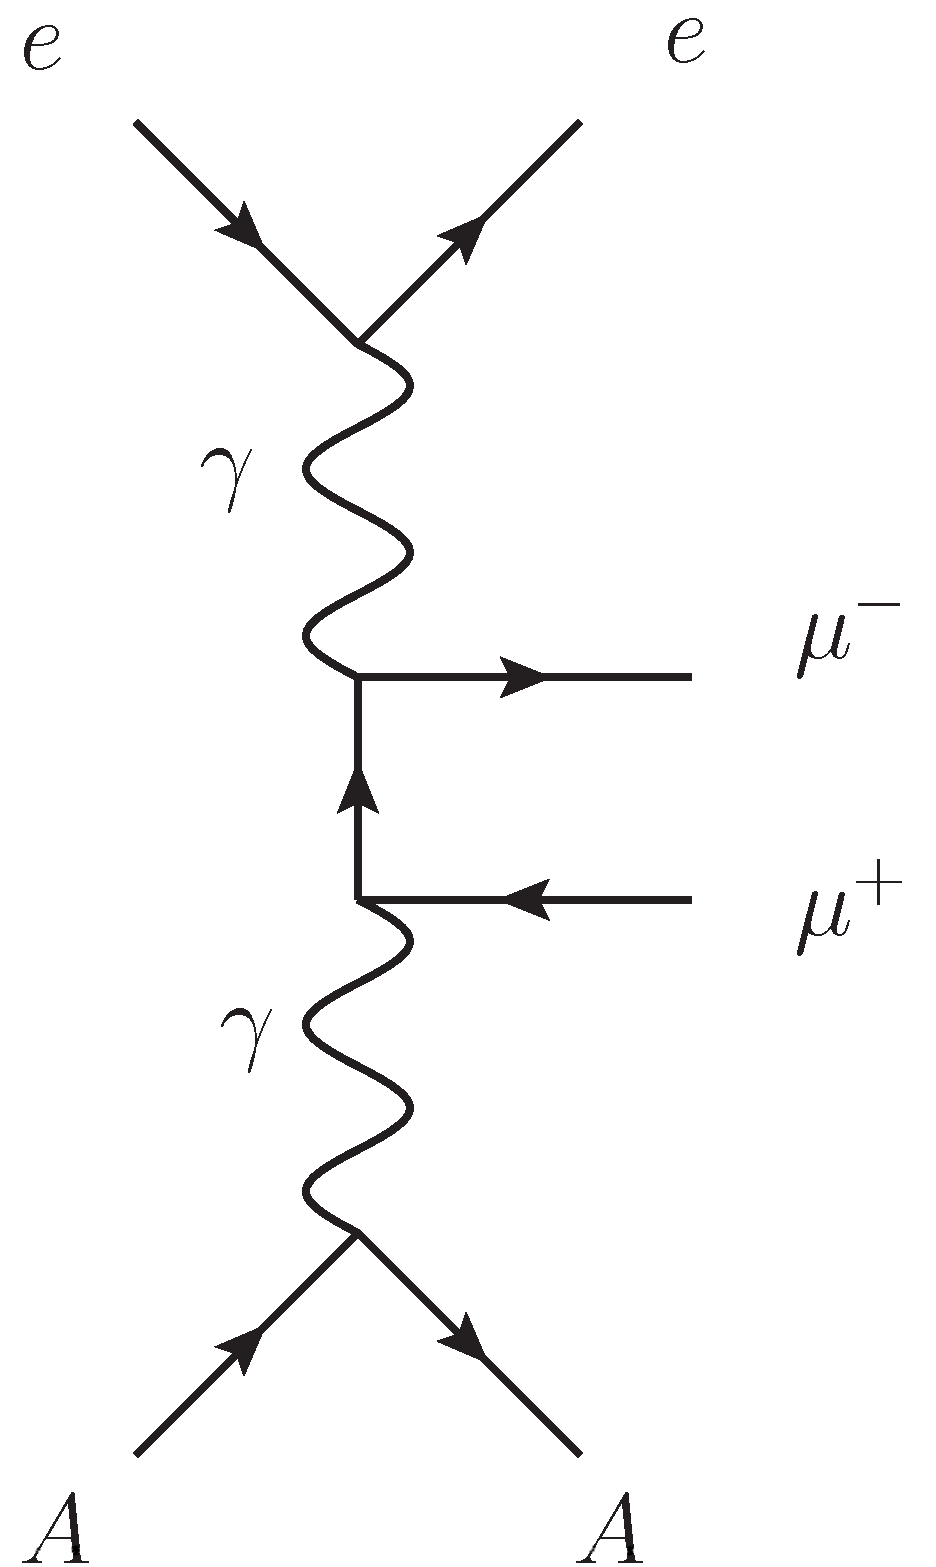
\includegraphics[width=0.5\textwidth]{Feynman_diagrams/Jaxo_BetheHeitler.png}
    \caption{Bethe-Heitler}
    \end{subfigure}\\
    \begin{subfigure}[b]{0.4\textwidth}\centering
    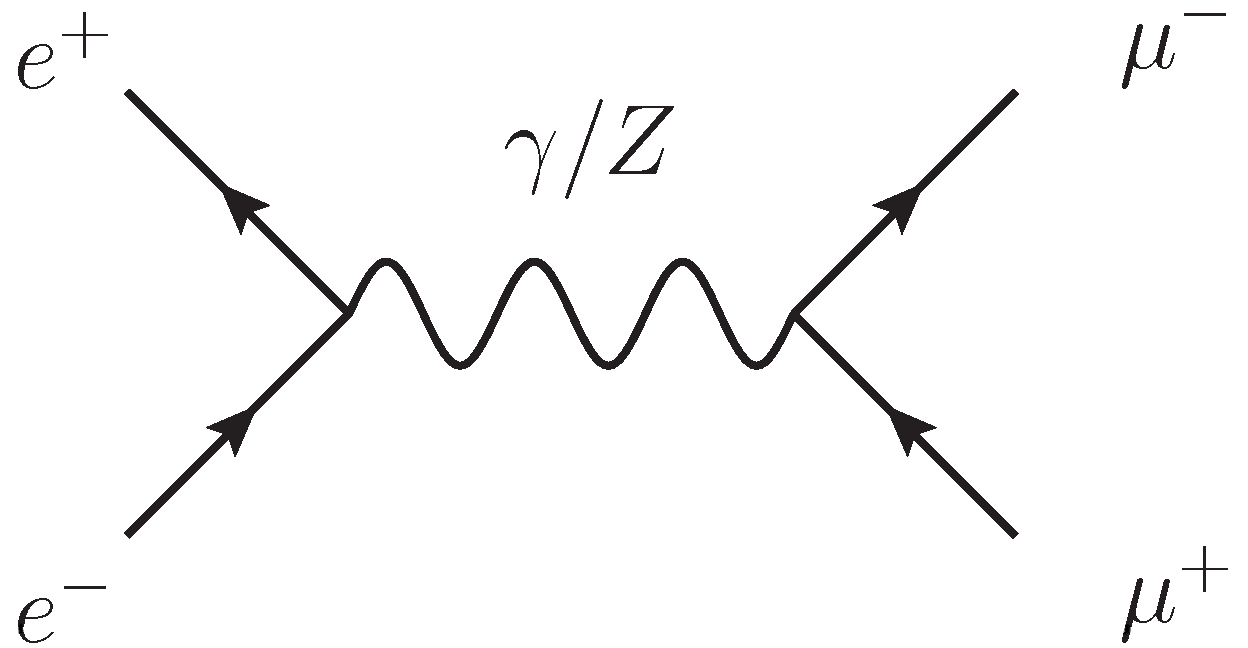
\includegraphics[width=0.7\textwidth]{Feynman_diagrams/Jaxo_annihilation.png}
     \caption{Direct annihilation}
     \end{subfigure}
    \caption[Muon production processes]{
    Feynman diagrams of the muon pair production via the Bethe-Heitler process and the direct annihilation with atomic electrons.}
    \label{fig:BDS_Muons:Muon_production}
\end{wrapfigure}
To prevent the muons from reaching the detectors, two different shielding systems are studied with respect to their effectiveness and feasibility to be integrated in the BDS.
Both systems are based on two ideas: to deflect the muons such that they do not reach the interaction region, and also to stop the muons in the shielding material.
The shielding scenarios that are under discussion foresee a combination of the two systems:
\begin{itemize}
 \item ``5 spoilers'':\\
 In the first scenario, five cylindrical spoilers out of magnetized iron are installed at different locations along the BDS: \SI{1358.5}{\metre}, \SI{1234.5}{\metre}, \SI{1145.5}{\metre}, \SI{975.5}{\metre}, and \SI{802.5}{\metre} from the interaction point (IP), where these locations indicate the midpoint of the spoiler.
 \\The spoilers have a radius of \SI{70}{\centi\meter}, and a length of about \SI{5}{\meter}.
 Their magnetic field ranges from about \SI{1.9}{\tesla} in the center of the spoiler to about \SI{1}{\tesla} at the outer edge~\cite{MuonShielding,Lewis}.
 An illustration of one of these spoilers is given in Figure~\ref{fig:BDS_Muons:shielding_options} (a).
 As indicated by the muon tracks through the spoiler, the magnetic field of the cylindrical spoilers is such that either positively or negatively charged muons are deflected away from the beam path into the tunnel walls.
 \item ``5 spoiler + wall'':\\
 In the second scenario, the same five spoilers are located at the same positions as before.
 But an additional magnetized shielding wall is placed about \SI{400}{\meter} from the interaction point.
 \\The wall is about \SI{5}{\meter} wide and long, and fills out the complete tunnel height.
 Its magnetic field strength is about \SI{1.6}{\tesla}~\cite{MuonShielding,Lewis}.
 Figure~\ref{fig:BDS_Muons:shielding_options} (b) shows an illustration of the wall inside the BDS tunnel.
\end{itemize}
The motivation for the study presented in this section is to investigate the effect of the muons on the \sid detector.
The overall goal is to give a recommendation, based on the study of the detector performance, on the necessity of the magnetized in order to keep the detector occupancy below the critical limit of \num{e-4} (as discussed in previous chapters).
Arguments against the wall were brought forward regarding costs and safety issues due to its size in the BDS tunnel.
 \begin{figure}
 \centering
  \begin{subfigure}[b]{0.49\textwidth}
   \centering
    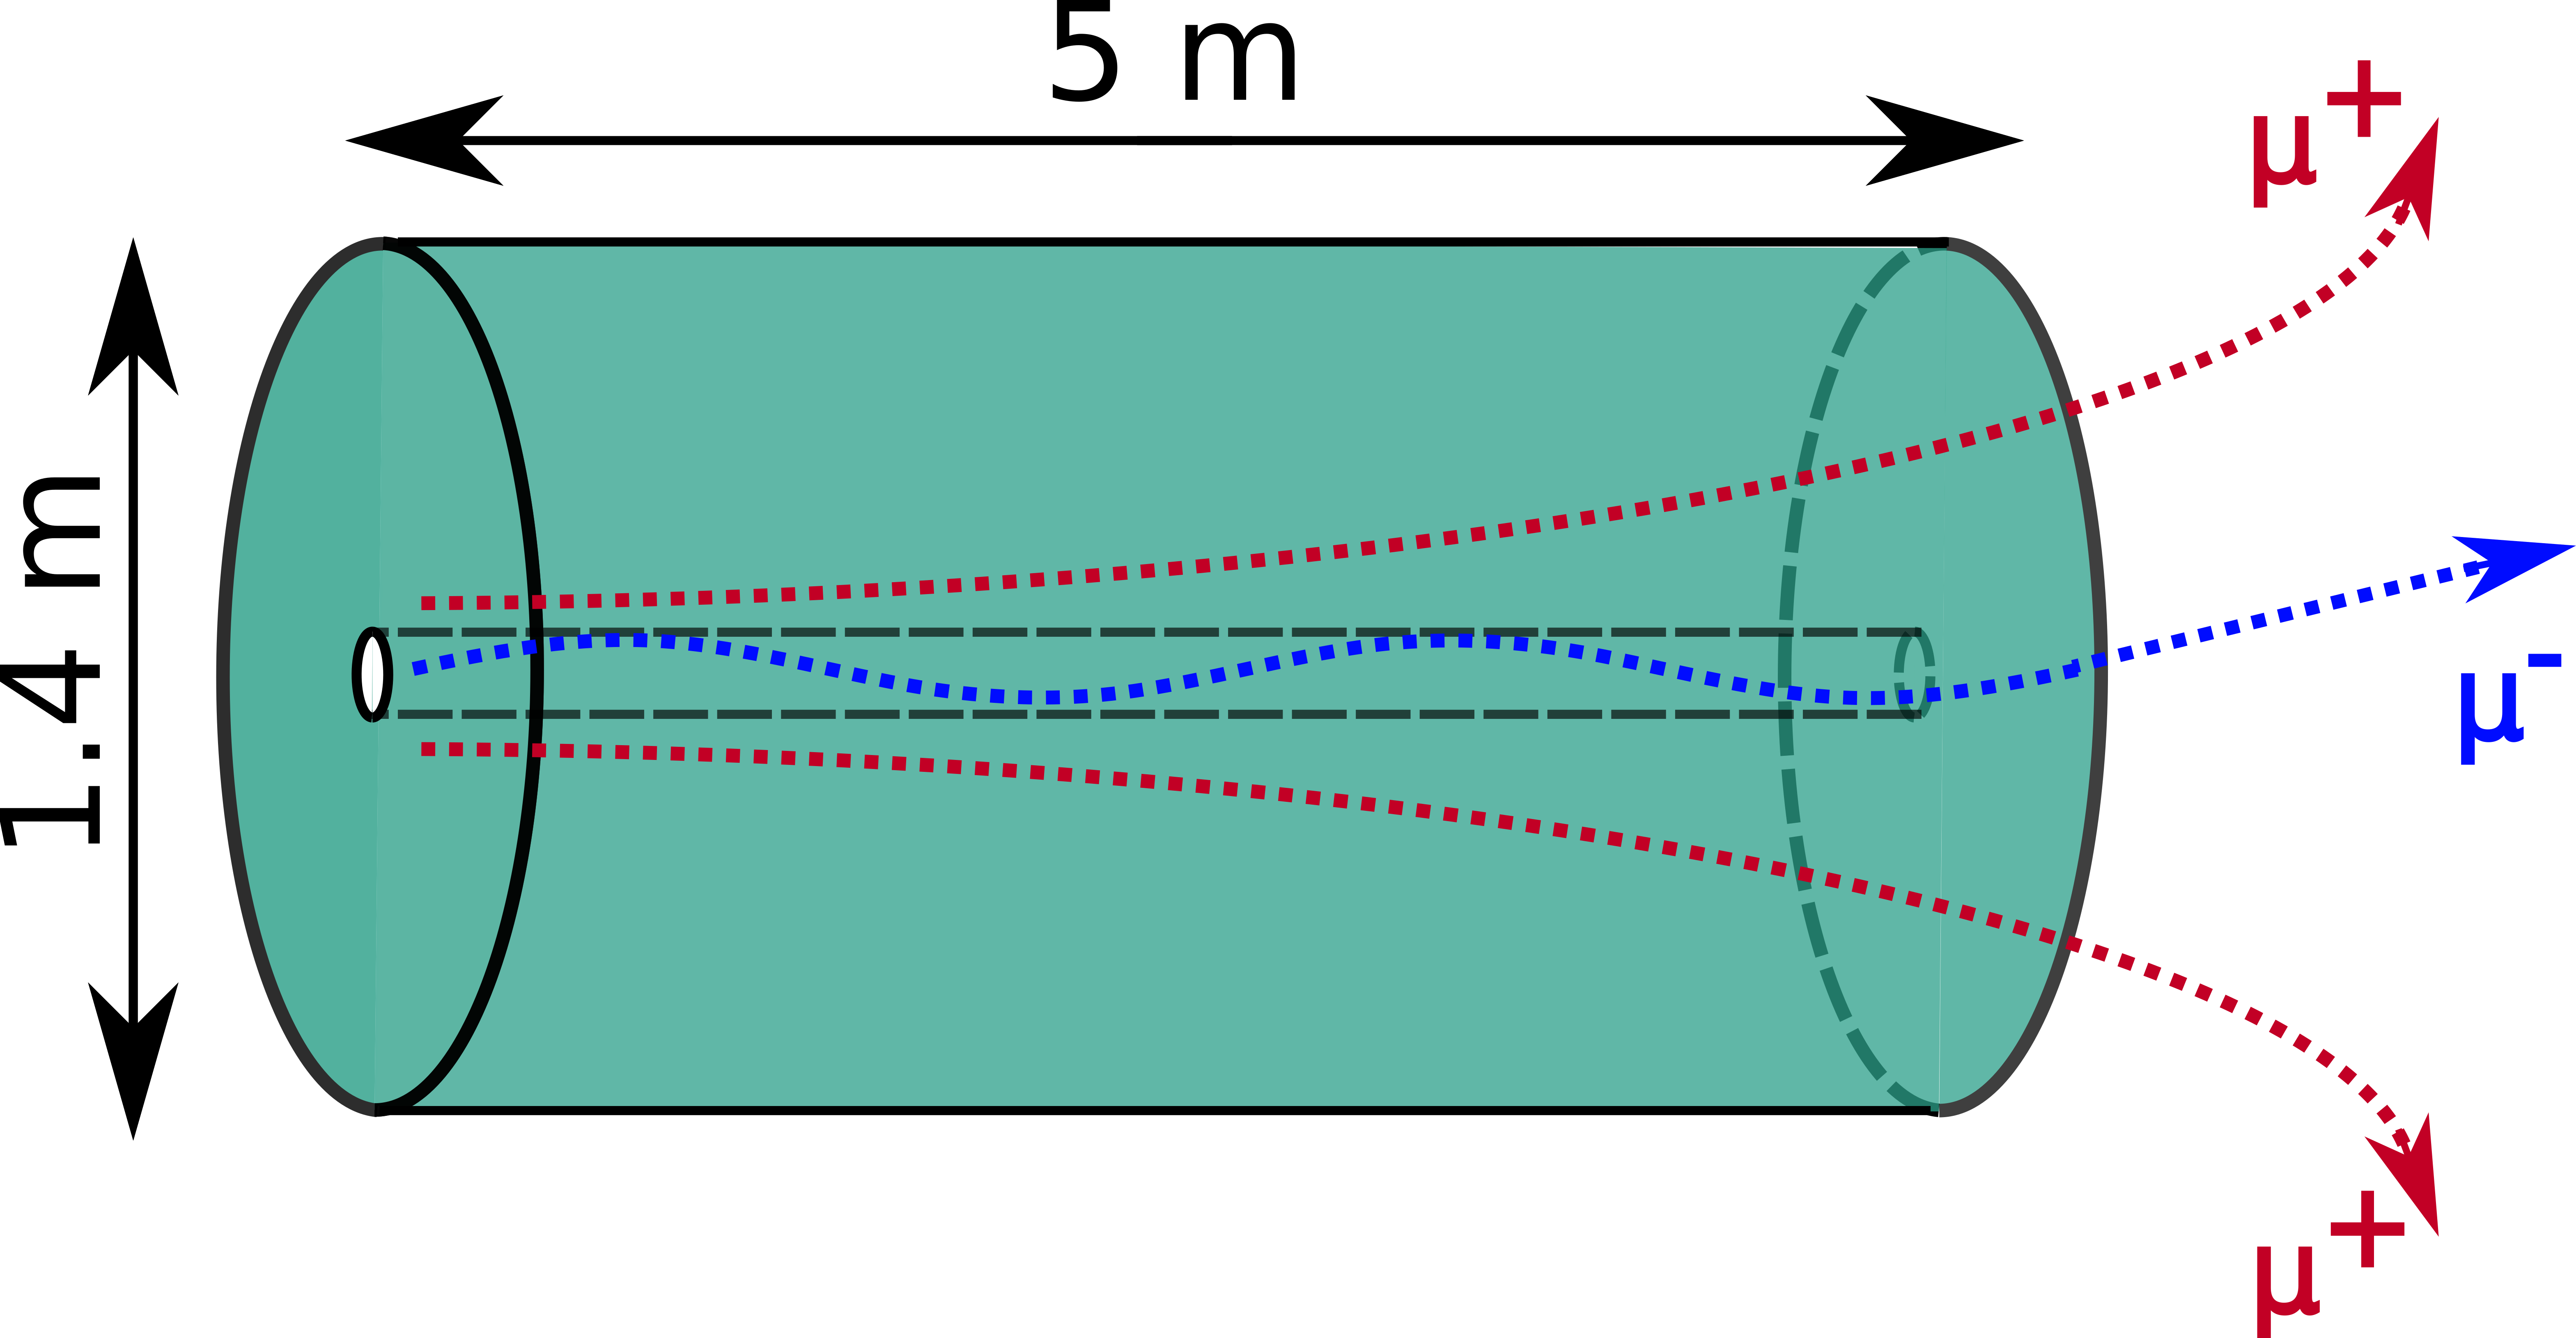
\includegraphics[width=0.7\textwidth]{Figures/BDS_muons/spoilers.png}
   \caption{Cylindrical spoiler}
   \label{fig:spoilers}
   \end{subfigure}
   \hfill
    \begin{subfigure}[b]{0.49\textwidth}
   \centering
    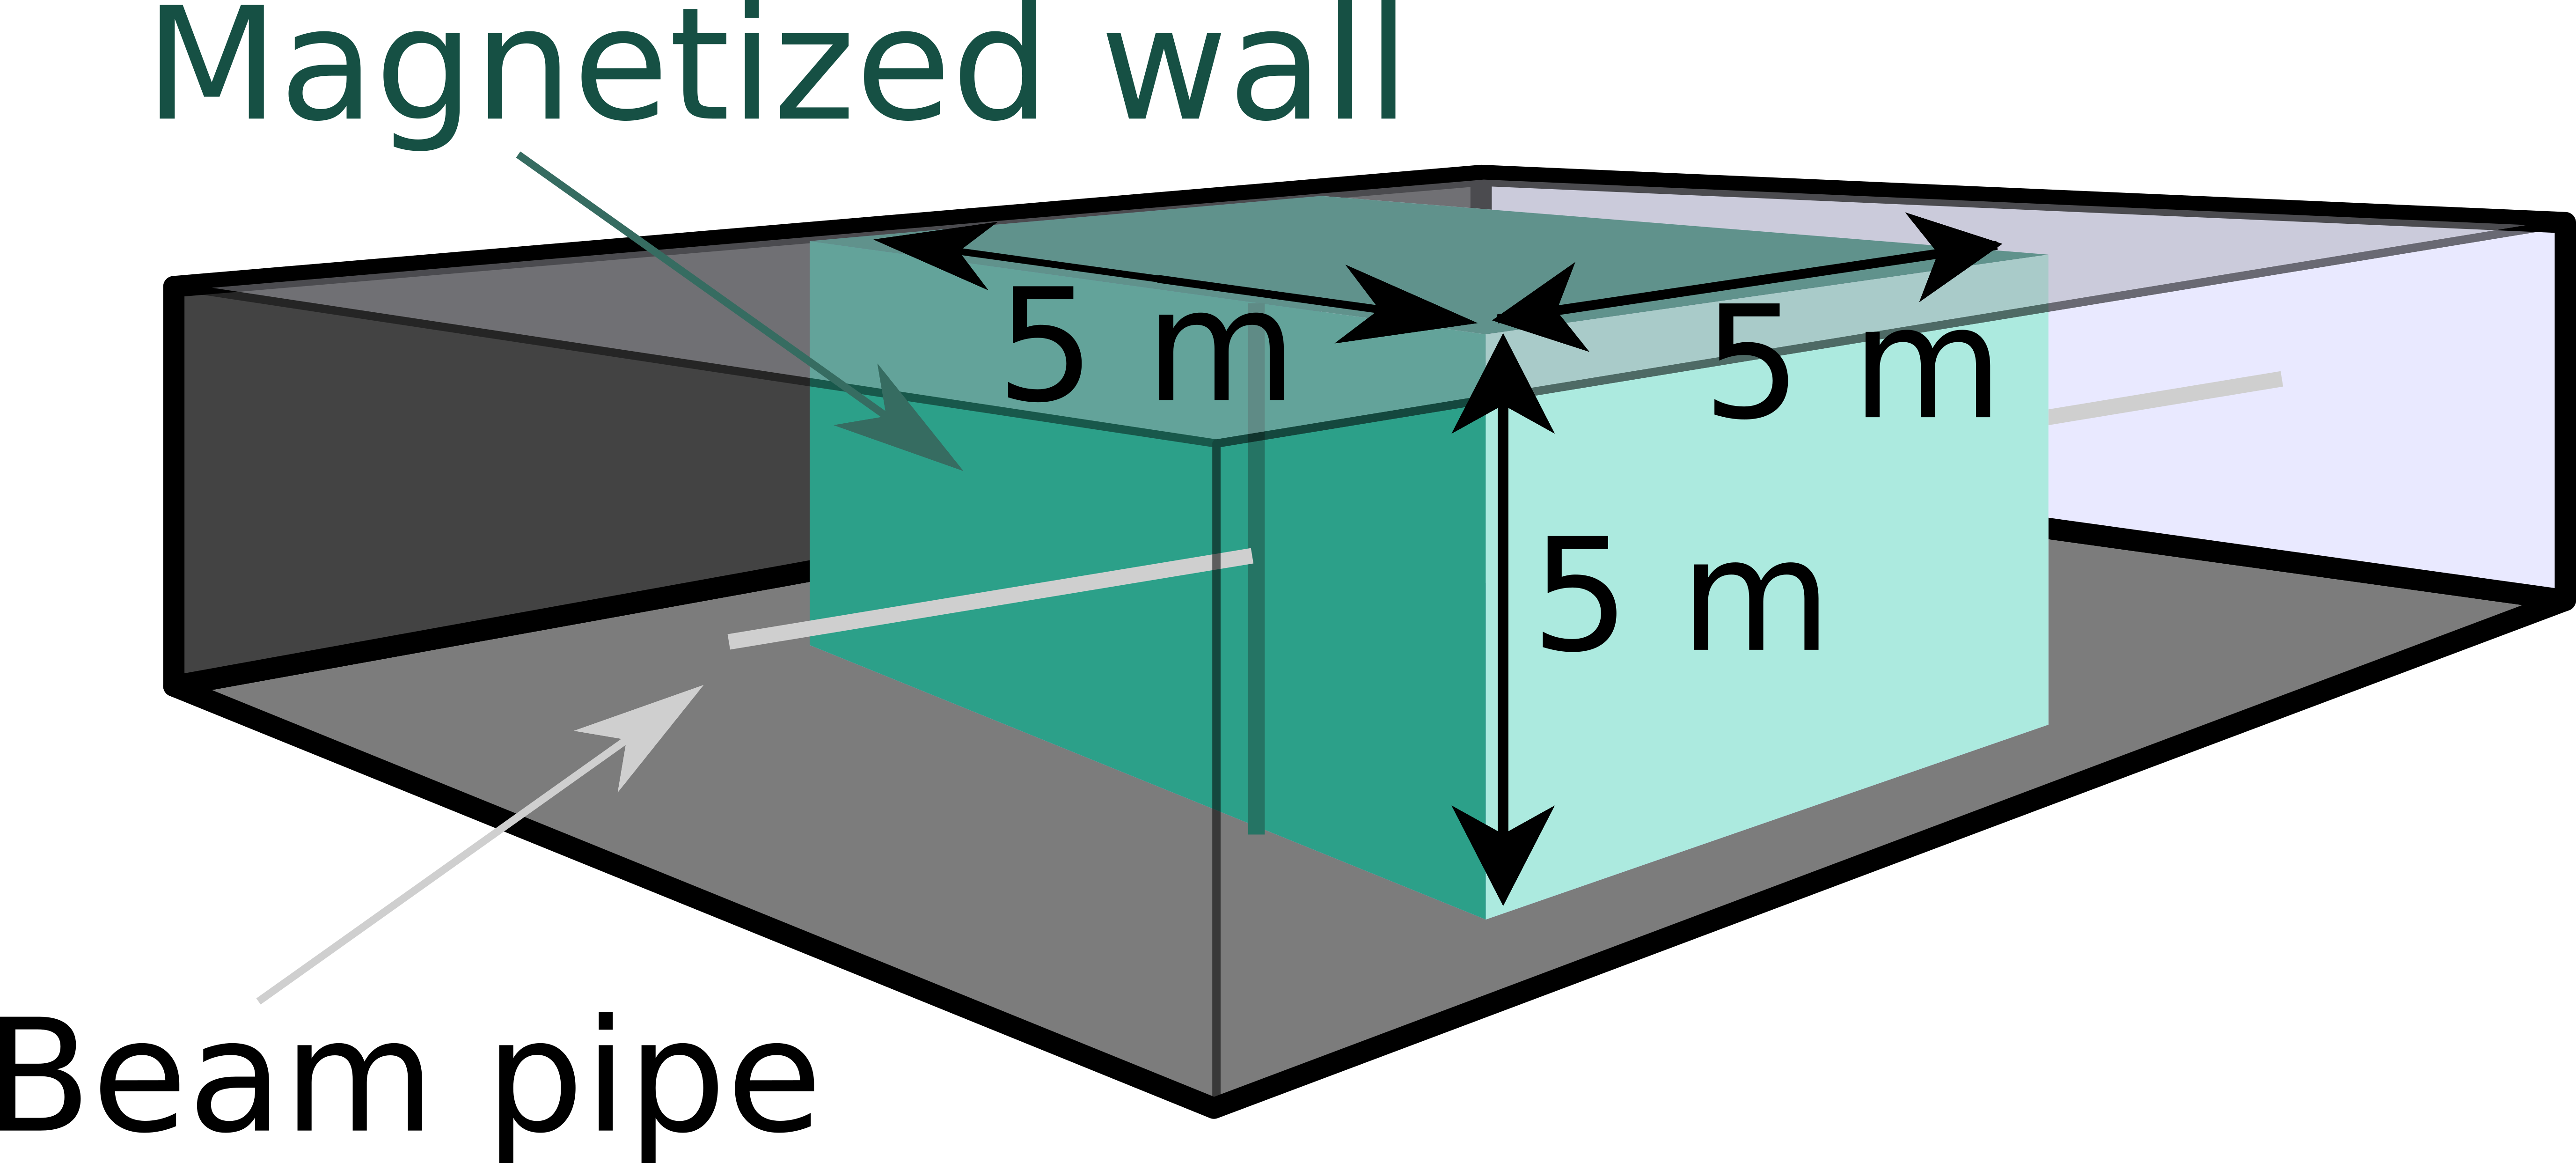
\includegraphics[width=\textwidth]{Figures/BDS_muons/muon_wall.png}
   \caption{Magnetized wall}
   \label{fig:muon_wall}
   \end{subfigure}
   \caption[BDS muon shielding options]{Schematic drawings of the magnetized spoiler (a) and the magnetized shielding wall (b)~\cite[cf. p. 2]{MuonShielding}.
   The magnetized wall is illustrated inside the accelerator tunnel.}
   \label{fig:BDS_Muons:shielding_options}
 \end{figure}

\section{\mucarlo}
\label{BDS_Muons:MUCARLO}
The interactions between the ILC beam and the machine components in the BDS were simulated with a Monte Carlo tool called \mucarlo~\cite{Mucarlo,MuonBkg_05TeV,MuonBkg_1TeV}.
Since the presented study is done for two different ILC stages, at \SI{250}{\GeV} and at \SI{500}{\GeV}, the beam parameters of the respective stage were used accordingly.
The geometry lattice of the ILC Beam Delivery System serves as the input geometry to the \mucarlo code, through which the muons are tracked.
Figure~\ref{fig:BDS_Muons:tracks} shows the muon tracks in the electron-line of the BDS.
The muons are created at certain locations along the beam line, are deflected by the magnetic field of beam line components, and lose kinetic energy through scattering in the material of the components the muons hit.
In the end, only those muons that reach the IP (at z = \SI{0}{\meter}) are stored.
Accordingly, Figure~\ref{fig:BDS_Muons:tracks} only shows those muons.
In this plot, there is only one red muon track line, which belongs to a negatively charged muon.
The spoiler polarities are set to defocus muons with the same charge as the beam charge.
Therefore, mainly positively charged muons from the electron beam line will reach the IP.
For the positron beam line, the muons reaching the IP are mainly negatively charged.
\\The main sources of muons were identified in the BDS to be 11 distinct collimators.
The following list names these collimators and their position from the IP~\cite{Lewis}:
\begin{itemize}
 \item Primary collimator spoilers (radiation length: 0.6 X\textsubscript{0}, half-gap\footnote{The term ``half-gap'' is commonly used for collimator systems.
 It describes the gap between one of the collimator jaws and an arbitrarily chosen plane (usually the beam center plane).
 Both of the jaws have the same distance from this plane.}: \SI{930}{\micro\meter} in x, \SI{400}{\micro\meter} in y):\\
  SP2 (\SI{1508}{\meter}), SP4 (\SI{1332}{\meter})
 \item Protection collimators (radiation length: 30 X\textsubscript{0}, inner radius: \SI{0.7}{\centi\meter}):\\
  PC1 (\SI{1452}{\meter}), PC2 (\SI{1387}{\meter}), PC5 (\SI{1276}{\meter}), PC5A (\SI{1242}{\meter}), PC6 (\SI{1208}{\meter}), PC7 (\SI{1047}{\meter})
 \item Absorbers (radiation length: 30 X\textsubscript{0}, half-gap: \SI{0.7}{\centi\meter}):\\
  AB3 (\SI{1420}{\meter}), AB5 (\SI{1237}{\meter}), ABE (\SI{852}{\meter})
\end{itemize}
The protection collimators and absorbers serve the purpose of protecting the magnets of the BDS from particle showers (arising from the beam halo collimation) and from mis-steered primary beams.
The number of muons created is proportional to the fraction of the collimator surface that is hit with respect to the beam size, which was determined with the help of the Monte Carlo ray-tracing computer program \turtle~\cite{Turtle}.
The general design of these collimators can be found in \cite{BDS_coll_design}.
\begin{figure}
\centering
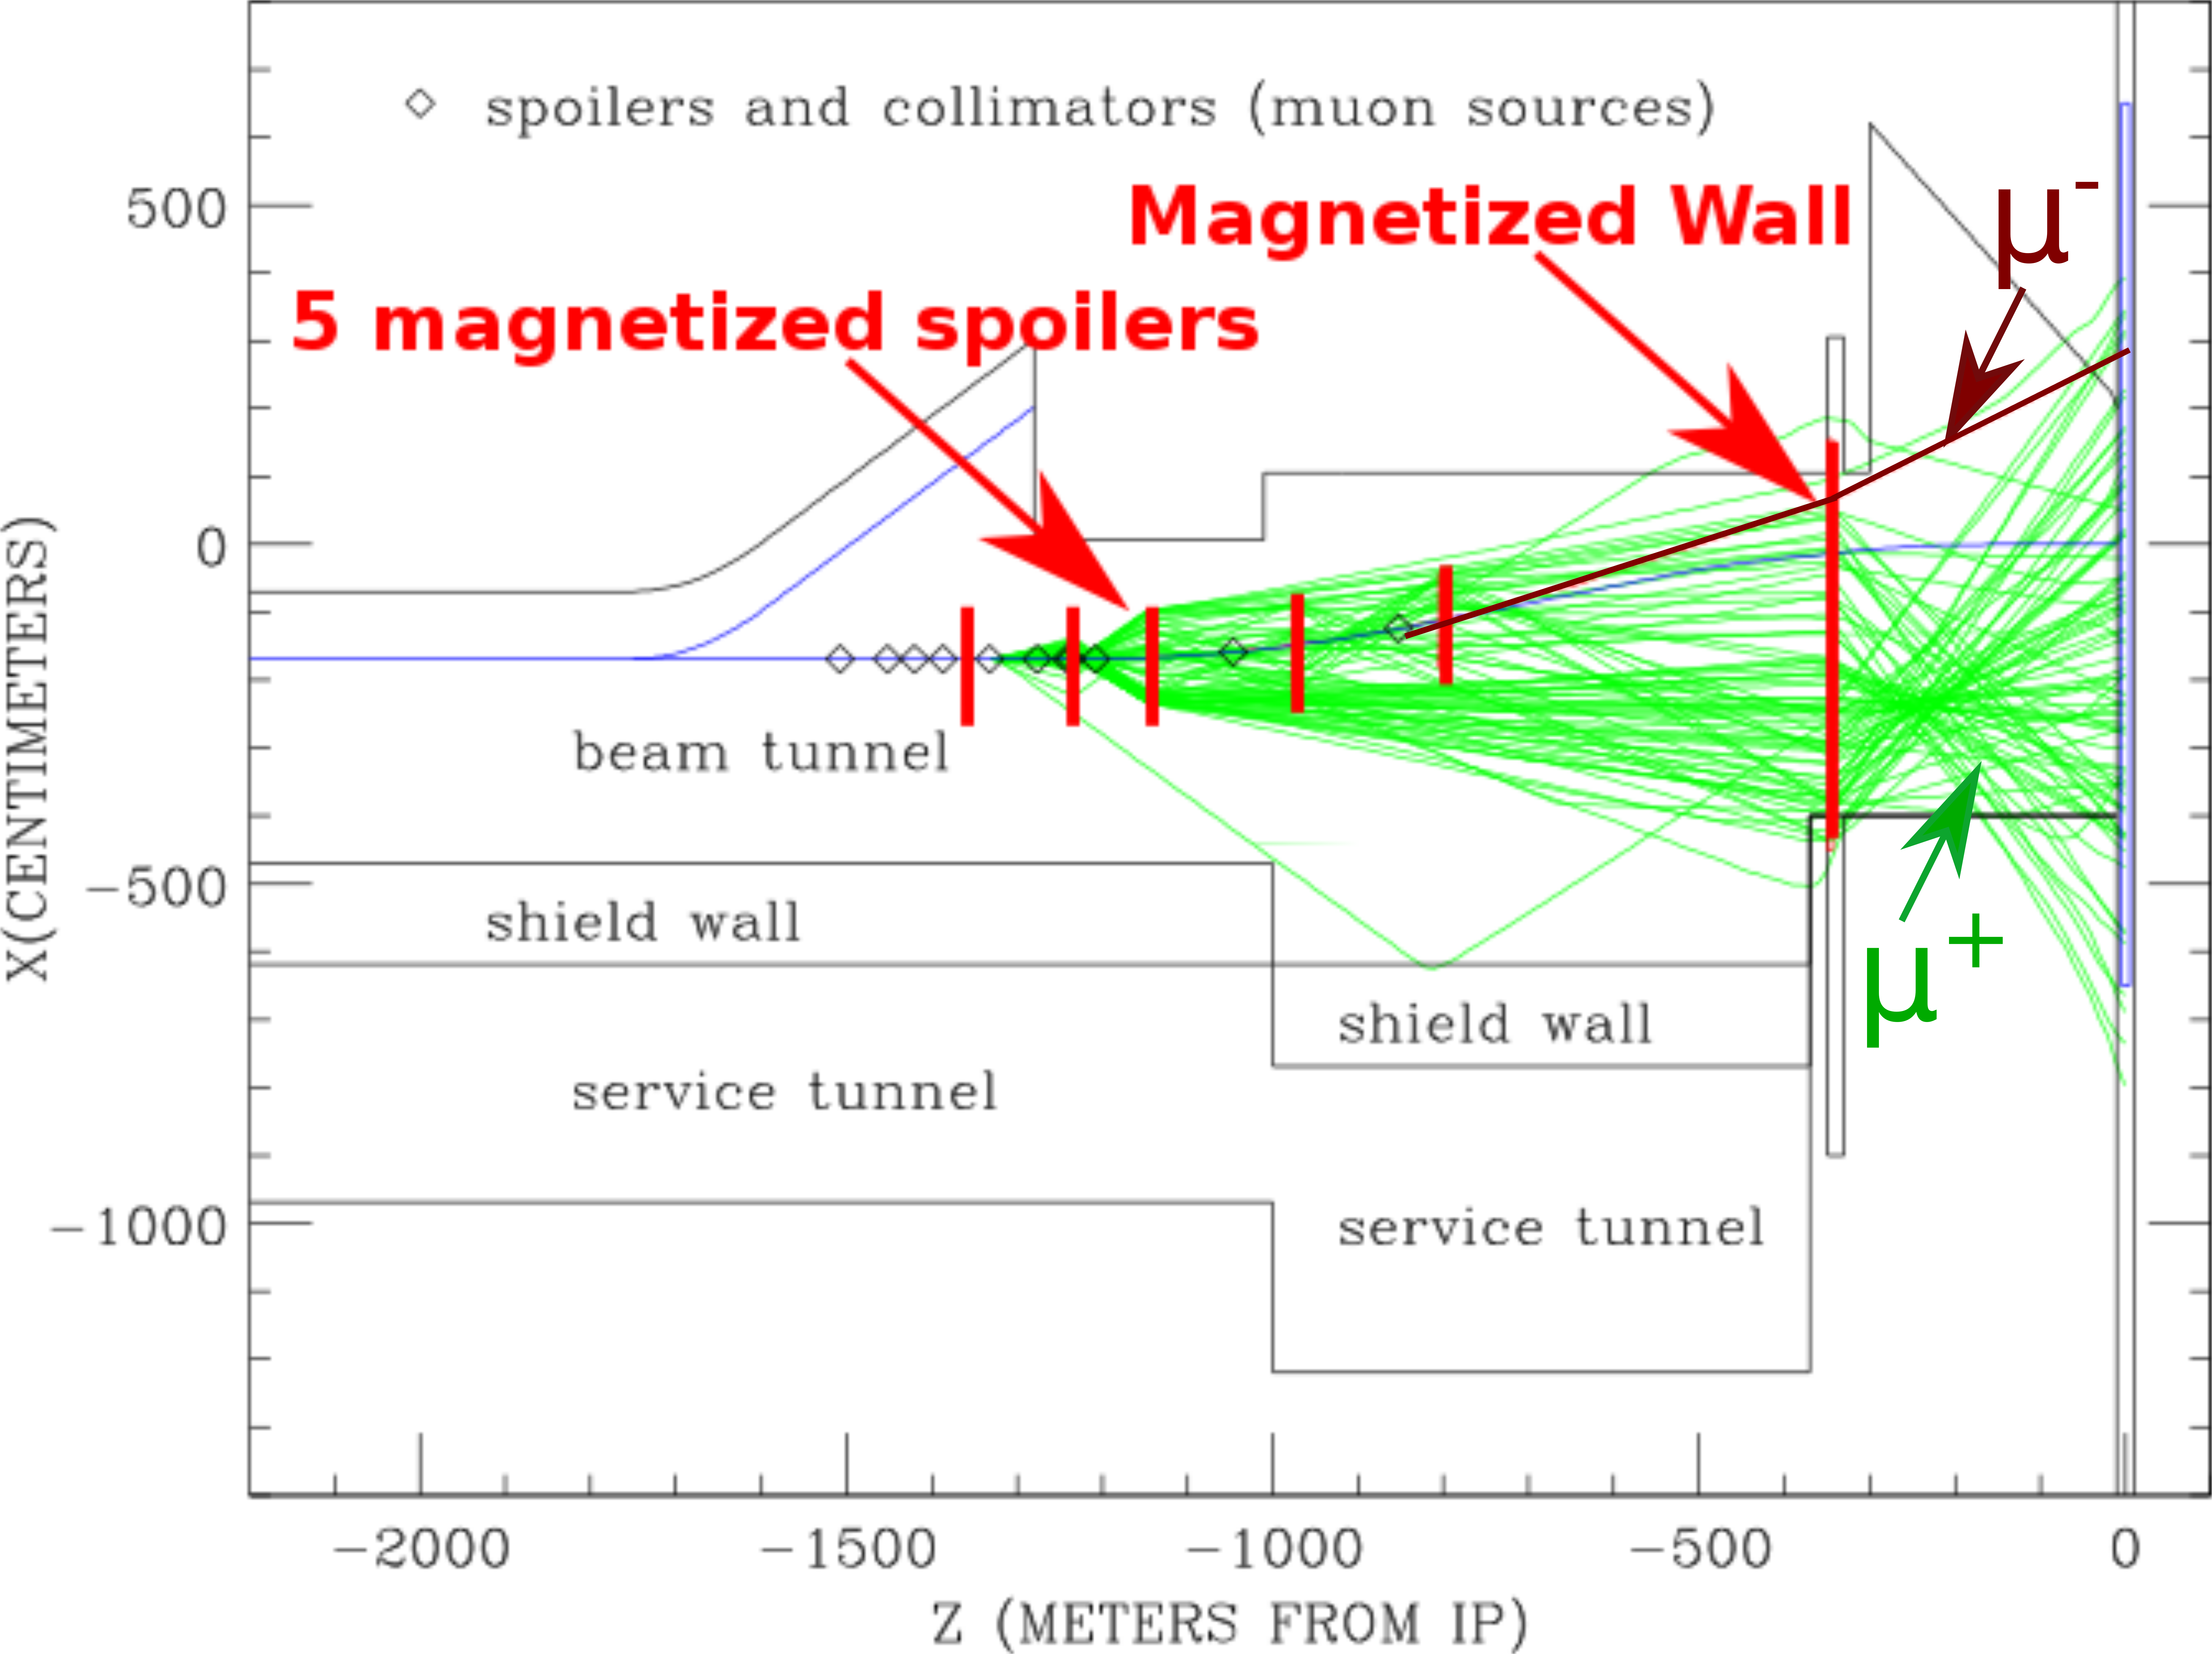
\includegraphics[width=0.6\textwidth]{Figures/BDS_muons/BDS_Tunnel_Spoilers+Wall_edited.png}
\caption[Muon tracks in the Beam Delivery Systems]{Visualization of the muon tracks in the ILC Beam Delivery System (BDS) in the electron beam line~\cite{Lewis}.
The picture shows the xz-plane of the BDS tunnel with the beam line components (spoilers and collimators), which serve as muon sources.
In this particular example, the muons origin from the electron beam hitting the primary collimator spoiler SP4.
The locations of the muon shielding components (the magnetized spoilers and wall) are also indicated.
The green/red thin lines represent the tracks of the muons.
\\The general layout of the tunnel model is the same for the electron and the positron beam line, but mirrored at the z = 0 plane.}
\label{fig:BDS_Muons:tracks}
\end{figure}
Adding up all muons from the different sources on the electron and the positron beam line side, the total number of muons can be calculated that would reach a detector with a radius of \SI{6.5}{\meter} at the interaction region.
Table~\ref{tab:BDS_Muons_muon_numbers} lists the muon rates per bunch crossing for a center-of-mass energy of 250 and \SI{500}{\GeV}, and for the two different shielding scenarios.
At \SI{500}{\GeV}, about 130 muons per bunch crossing would reach the detector in the case that no shielding was installed.
This number is reduced to about 4 muons with the five cylindrical spoilers, and to below 1 muon per bunch crossing with an additional magnetized wall.
For a lower beam energy of \SI{125}{\GeV} (\SI{250}{\GeV} center-of-mass energy), the number of muons that are produced is lower, because of which only around 38 muons reach the detector without shielding.
With the two different shielding scenarios, the muon rate is again reduced significantly to a minimum of about 0.03 per bunch crossing.
%------------------
%\newcolumntype{L}[1]{>{\raggedright\let\newline\\\arraybackslash\hspace{0pt}}m{#1}}
\newcolumntype{C}[1]{>{\centering\let\newline\\\arraybackslash\hspace{0pt}}m{#1}}
%\newcolumntype{R}[1]{>{\raggedleft\let\newline\\\arraybackslash\hspace{0pt}}m{#1}}
%-----------------
\begin{table}[htbp]
\caption[\mucarlo muon rates]{Muon rates per bunch crossing for the two shielding scenarios, gained from \mucarlo simulations~\cite{Lewis}.}
\label{tab:BDS_Muons_muon_numbers}
\centering
\begin{tabularx}{0.8\textwidth}{l|C{1.4cm}C{1.4cm}C{1.4cm}|C{1.4cm}C{1.4cm}C{1.4cm}}
\hline\hline
\textbf{Scenario} & \multicolumn{6}{>{\centering}p{10cm}}{\textbf{Muons per bunch crossing in a detector with 6.5\,m radius}}\\
& \multicolumn{3}{>{\centering}p{5cm}}{ILC500} & \multicolumn{3}{>{\centering}p{5cm}}{ILC250}\\
& positron line & electron line & total & positron line & electron line & total\\
\hline
 No Spoilers & 71.6 & 58.5 & 130.1 & 21,1 & 17,2 & 38.3\\
 5 spoilers& 2.3 & 2 & 4.3 & 0.73 & 0.57 & 1.3\\
 5 spoilers + wall & 0.34 & 0.26 & 0.6 & 0.016 & 0.014 & 0.03\\
\hline\hline
\end{tabularx}
\end{table}
\\The output of \mucarlo is a text file containing the four-vectors of the muons \SI{10}{\meter} from the IP.
These four-vectors can therefore be used as input to a full detector simulation. 
\\An additional study was done using a \geant simulation of the BDS tunnel in order to cross check the \mucarlo results and to thereby verify the \mucarlo simulation.
The outcome of that study was that both simulations are in good agreement~\cite{Glens_muon_talk}.

\section{Effect of muons on the \sid performance}
\label{BDS_Muons:SiD}
Since the \sid detector only reads out the hits after every bunch train (1312 bunch crossings), the detector occupancy for the muons has to be studied for a muon rate per train.
As in the previous chapter, the full detector simulation was done using \slic.
The geometry input file that was used contained the most recent sidloi3 geometry of the \sid detector, including the new L* position, the anti-DiD field, as well as the Pacman geometry.
For details on these detector characteristics, please refer to Section~\ref{ILC:SiD}.
After a file-format conversion, the \mucarlo output files containing the four-vectors of the muons for the different shielding scenarios and center-of-mass energies served as the particle source input to \slic.

\subsection{Muon hit distribution}
\label{BDS_Muons:hit_time_dis}
For visualizing the hit distribution in the \sid detector, event displays (see Figure~\ref{fig:BDS_Muons:wired4}) were made using WIRED4~\cite{Wired4}.
 \begin{figure}[htbp]
 \captionsetup[subfigure]{justification=centering}
 \centering
  \begin{subfigure}[b]{0.4\textwidth}
   \centering
   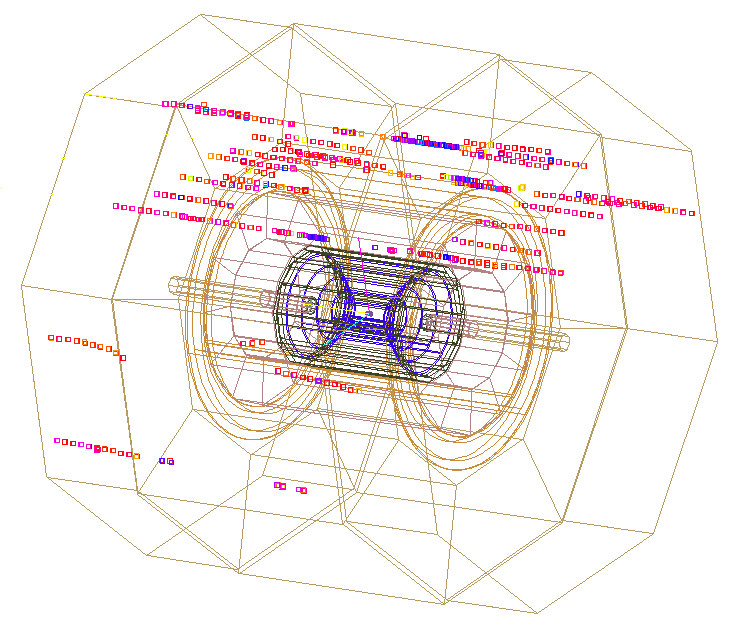
\includegraphics[width=\textwidth]{Figures/BDS_muons/Event_display_ILC250_p_spoilers_wall_inverted.png}
   \caption{3D view, 5 spoilers + wall,\\ILC250}
   \end{subfigure}\\
   \begin{subfigure}[b]{0.4\textwidth}
   \centering
    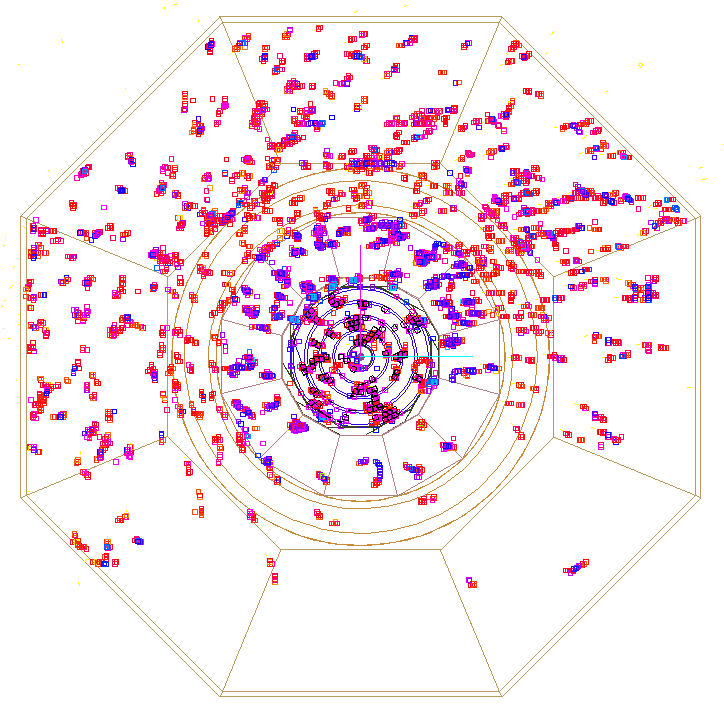
\includegraphics[width=0.9\textwidth]{Figures/BDS_muons/muons_positron_5spoilers_wall_515_xyview_croped_inverted.png}
   \caption{xy-view, 5 spoilers + wall,\\ILC500}
   \end{subfigure}
   \hfill
    \begin{subfigure}[b]{0.4\textwidth}
   \centering
    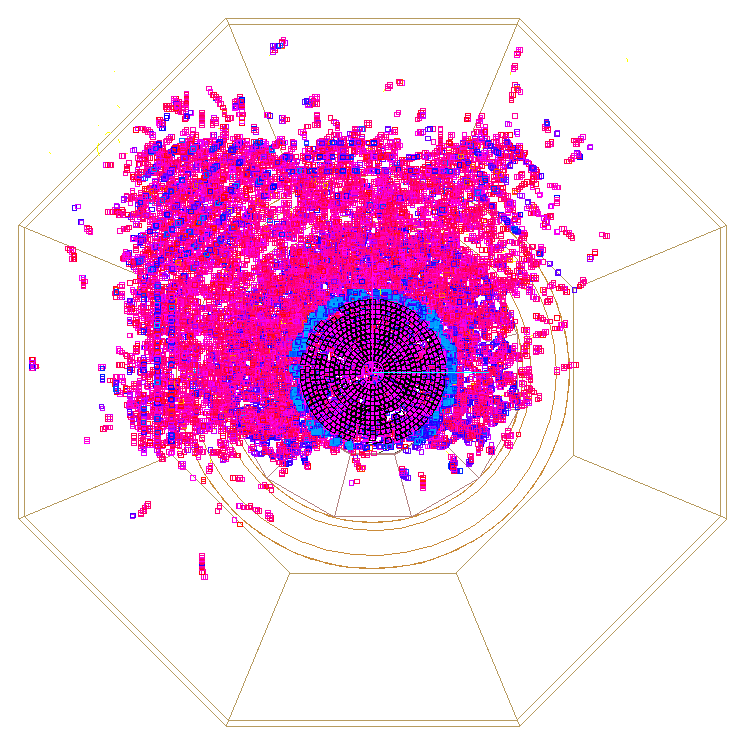
\includegraphics[width=0.9\textwidth]{Figures/BDS_muons/muons_positron_5spoilers_2961_xyview_croped_inverted.png}
   \caption{xy-view, 5 spoilers,\\ILC500}
   \end{subfigure}
   \caption[Event displays of BDS muons in \sid]{Event displays of the muon hits in \sid for different center-of-mass energies and different shielding scenarios.}
   \label{fig:BDS_Muons:wired4}
 \end{figure}
\\Apart from the overall number of hits in the different event displays, the spatial distribution of the hits is striking.
Concentrating on Figure~\ref{fig:BDS_Muons:wired4} (a) first, the muons leave clear horizontal tracks throughout the whole detector.
After leaving the BDS tunnel, the muons (which are boosted in forward direction) enter \sid through the outermost subdetector, and penetrate the full detector.
Since the muons are coming from both the electron and the positron beam line, this happens simultaneously from both sides.
\\The difference in the spatial distribution in the xy-plane between Figure~\ref{fig:BDS_Muons:wired4} (b) and (c) is explained by the geometry of the tunnel, and position of the detector with respect to the tunnel exit.
In subfigure (a), the rectangular shape in the hit distribution is the imprint of the tunnel.
The boosted muons exit the tunnel and directly hit the detector.
The asymmetry of the imprint results from the position of the detector.
The beam pipe and therefore the central axis through the detectors are not in the center of the BDS tunnel.
As can be seen in Figure~\ref{fig:BDS_Muons:tracks}, the beam line curves such that it is closer to one of the tunnel side walls than to the other.
The top-bottom asymmetry is due to the fact that the detector cavern is below ground level of the tunnel.
\\Adding the magnetized wall as an additional muon shielding causes the muons to scatter.
The clear tunnel imprint is no longer visible in Figure~\ref{fig:BDS_Muons:wired4} (b).
Scattering the muons is not the only effect of the magnetized wall.
As can be seen in Figure~\ref{fig:BDS_Muons:energy}, the wall shifts the muon energy to lower values for a respective center-of-mass energy.
The muons are deflected away from the forward directions due to the magnetization of the wall, but also lose their energy in the material of the wall.
Low energy muons are either stopped completely, or deflected such that they cannot reach the detector. %\todo{Check out Bethe-Bloch here}
The peak in the energy distributions at lower energies is therefore reduced for the ``5 spoilers + wall'' scenarios.
Additionally, the number of muons per bunch train can directly be compared for the two ILC stages and the different shielding options.
\begin{figure}[htbp]
\centering
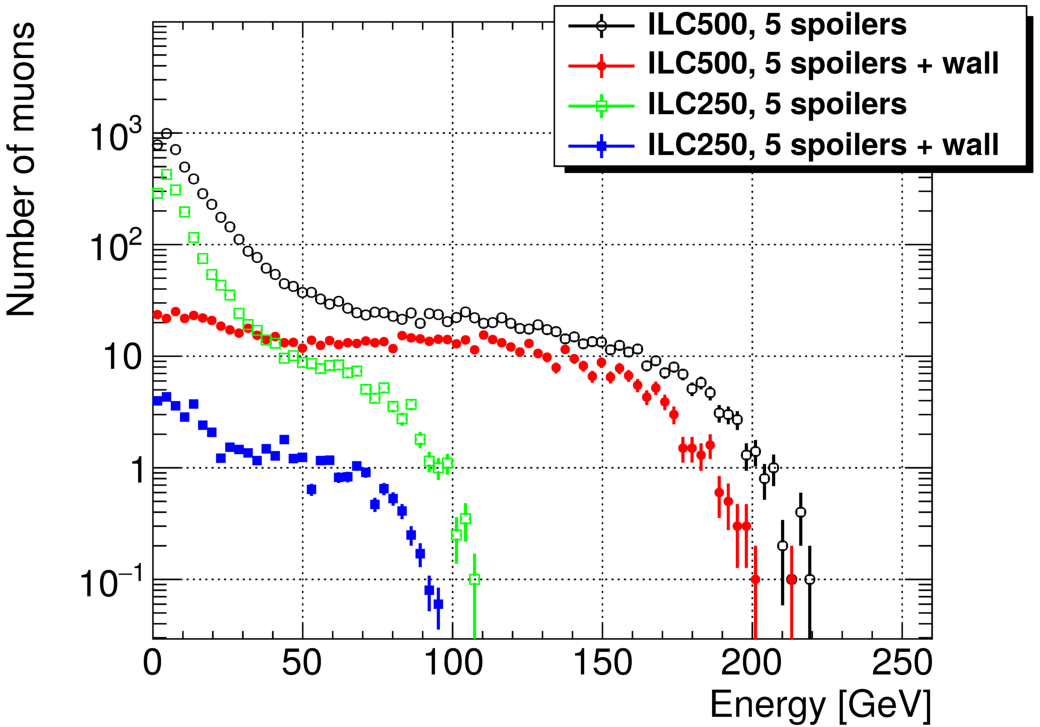
\includegraphics[width=0.6\textwidth]{Figures/BDS_muons/Energy_Comparison_ILC500vsILC250.pdf}
\caption[Muon energy]{Energy distribution of the muons for the different shielding scenarios, and for a center-of-mass energy of 250 and \SI{500}{\GeV}.
The number of muons are normalized to a full bunch train for all cases.}
\label{fig:BDS_Muons:energy}
\end{figure}
\\These muons then leave a particular number of hits in the \sid subdetectors by penetrating the full detector.
For the comparison between the total number of hits in the four different cases, Figure~\ref{fig:BDS_Muons:hits} shows a bar chart of the hits collected in each subdetector.
The largest number of hits is counted for the endcaps of the muon detector system, which is the subdetector with the largest effective detector area under normal incident of the muons.
Also, it is the outermost subdetector, likely to be hit by all of the primary muons.
Accordingly, the vertex detector (as the smallest and innermost detector) is hit the least number of times, and in the same manner also the other subdetectors gain representative number of hits.
Deducing from the hit distributions, the \sid detector will overall suffer from less hits in the ILC250 stage with respect to the ILC500, but adding the magnetized wall to the shielding will yield even smaller hit counts for both center-of-mass energies.
\begin{figure}[h]
\centering
\begin{subfigure}[t]{0.49\textwidth}
\centering
 \includegraphics[width=\textwidth]{Figures/BDS_muons/Hits_in_SiD_subdetectors_MuonSpoilerStudy_ILC250.pdf}
 \caption{ILC250}
\end{subfigure}
\begin{subfigure}[t]{0.49\textwidth}
\centering
 \includegraphics[width=\textwidth]{Figures/BDS_muons/Hits_in_SiD_subdetectors_MuonSpoilerStudy_ILC500.pdf}
  \caption{ILC500}
\end{subfigure}
\caption[Number of muon hits in the \sid subdetectors]{Total number of hits in the various \sid subdetectors for both shielding scenarios in the ILC250 stage (a) and ILC500 stage (b).
The number of hits come from muons from a full bunch train.}
\label{fig:BDS_Muons:hits}
\end{figure}
\\After looking at the total number of hits, which reflects the size and position of the subdetectors in \sid, this fact can be even better derived from the hit time distributions shown in Figure~\ref{fig:BDS_Muons:hittime}.
The muons emitted from the BDS tunnel arrive first at the endcaps of the muon system, as mentioned above.
After penetrating all muon endcap layers, the next outermost subdetector is hit and so on, until the muons make their way to the opposite muon endcap.
The time needed for the muons to penetrate the full detector is hence about \SI{40}{\nano\second}, independent of the muon shielding and the center-of-mass energy.
\begin{figure}[htbp!]
\centering
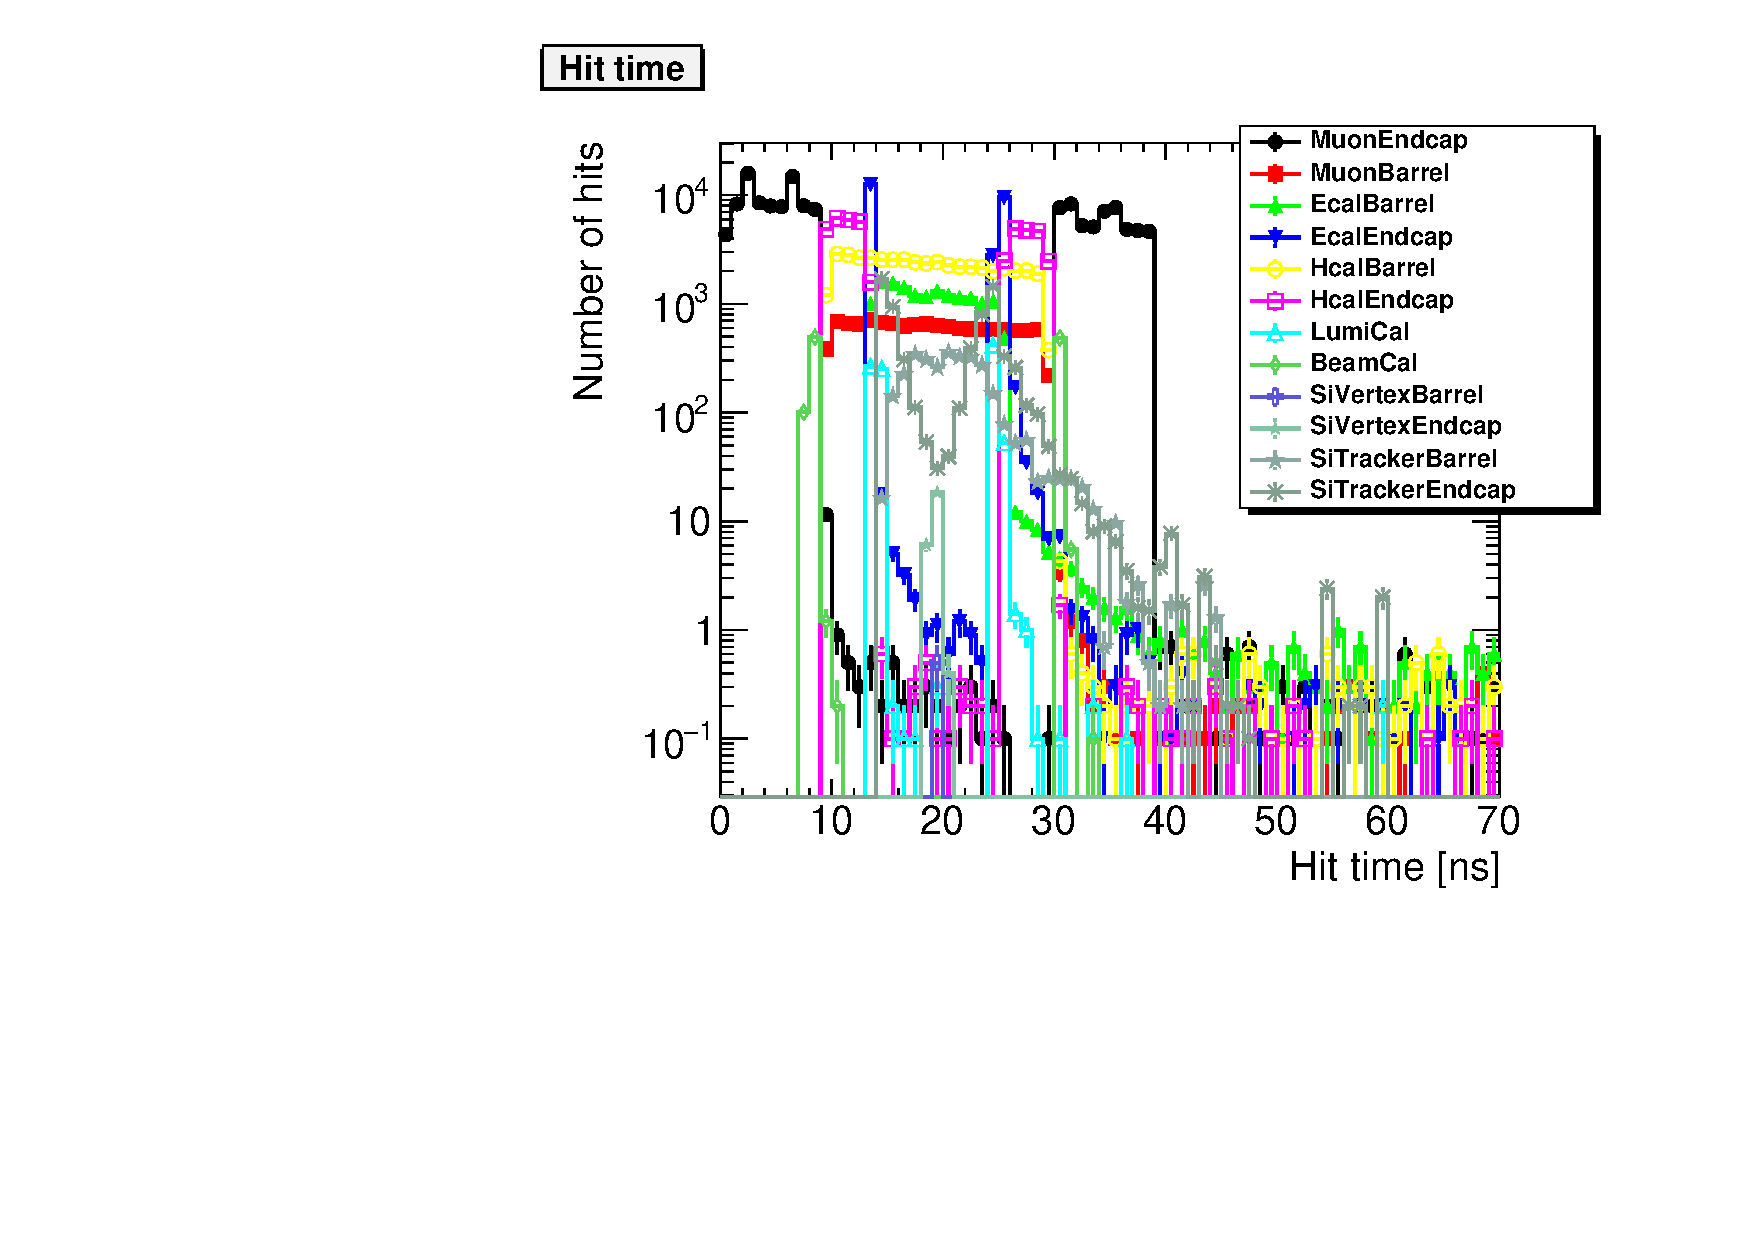
\includegraphics[width=0.7\textwidth]{Figures/BDS_muons/hittime_ILC500_spoilers_superimposed.pdf}
\caption[Muon hit time in the \sid subdetectors]{Hit time distribution of the BDS muons in the various \sid subdetectors for ILC500 stage and for the ``5 spoilers'' scenario only.
The number of hits are normalized to hits from a full bunch train for all cases.}
\label{fig:BDS_Muons:hittime}
\end{figure}

\subsection{\sid occupancy}
\label{BDS_Muons:sidocc}
The next step is to look at the occupancy of the detector arising from these muon hits.
As in Chapter~\ref{PairBkg:occupancy}, the number of hits are counted for every cell in the subdetectors, which can be directly translated into a detector occupancy.
In the following, the muon occupancy in the \sid HCAL barrel and the tracker endcaps is discussed.
As explained in the previous chapter, occupancy plots show how many detector cells are hit a certain number of times. 
By respecting the rule that the sum of all cells with a number of hits greater than or equal to the buffer depth should not exceed \SI{0.01}{\percent} (\num{e-4} of all cells), a statement can be made whether given occupancy levels are acceptable.
By optimizing the design of the detectors and the accelerator, a balance can be found between a sufficient buffer depth of the detector sensors and low background levels arising from the accelerator.
\\Figure~\ref{fig:BDS_Muons:HcalBarrel} shows the occupancy and the number of dead cells~\footnote{A cell is defined to be dead when the buffer of its sensor is already completely filled, and no further hits can be stored. Further details can be found in Chapter~\ref{PairBkg:occupancy}.} in the HCAL barrel, normalized to its total number of cells.
In the current detector design, the HCAL cells have a size of \SI{1}{\centi\meter}$\times$\SI{1}{\centi\meter}.
As a result, a maximum of three hits per cell is observed, because of which the x-axis range in Figure~\ref{fig:BDS_Muons:HcalBarrel} (b) also reaches to three only.
Here, the number of dead cells is shown as a function of the assumed buffer depth.
In the theoretical case of a buffer depth of one, about \num{e-4} of all cells would have a full buffer (with one hit) for the ``5 spoilers'' case in the ILC500.
Here, the critical limit for acceptable occupancies of \num{e-4} would just about be reached, all other cases would have acceptable values.
Realistically, the HCAL sensor will have a higher buffer depth, namely a buffer depth of four (in the current design) or higher.
Since none of the cells are hit by more than three muons, the occupancy in the HCAL barrel is very low and far from the critical limit.
 \begin{figure}
 \centering
  \begin{subfigure}[b]{0.49\textwidth}
   \centering
    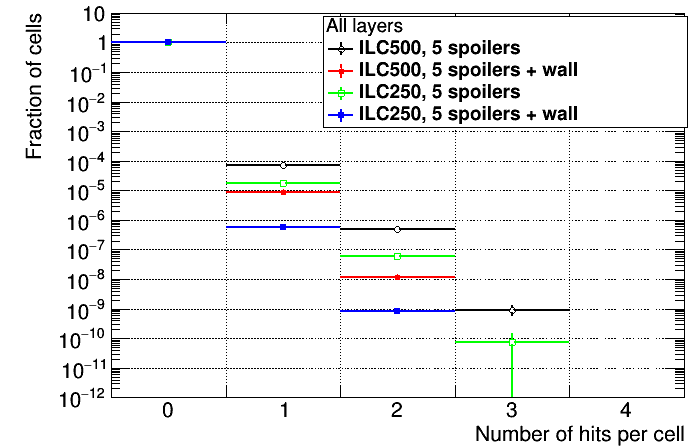
\includegraphics[width=\textwidth]{Figures/BDS_muons/Occupancy_Comparison_All_layers_wrt_cells_HcalBarrel.png}
   \caption{Normalized occupancy}
   \end{subfigure}
   \hfill
    \begin{subfigure}[b]{0.49\textwidth}
   \centering
    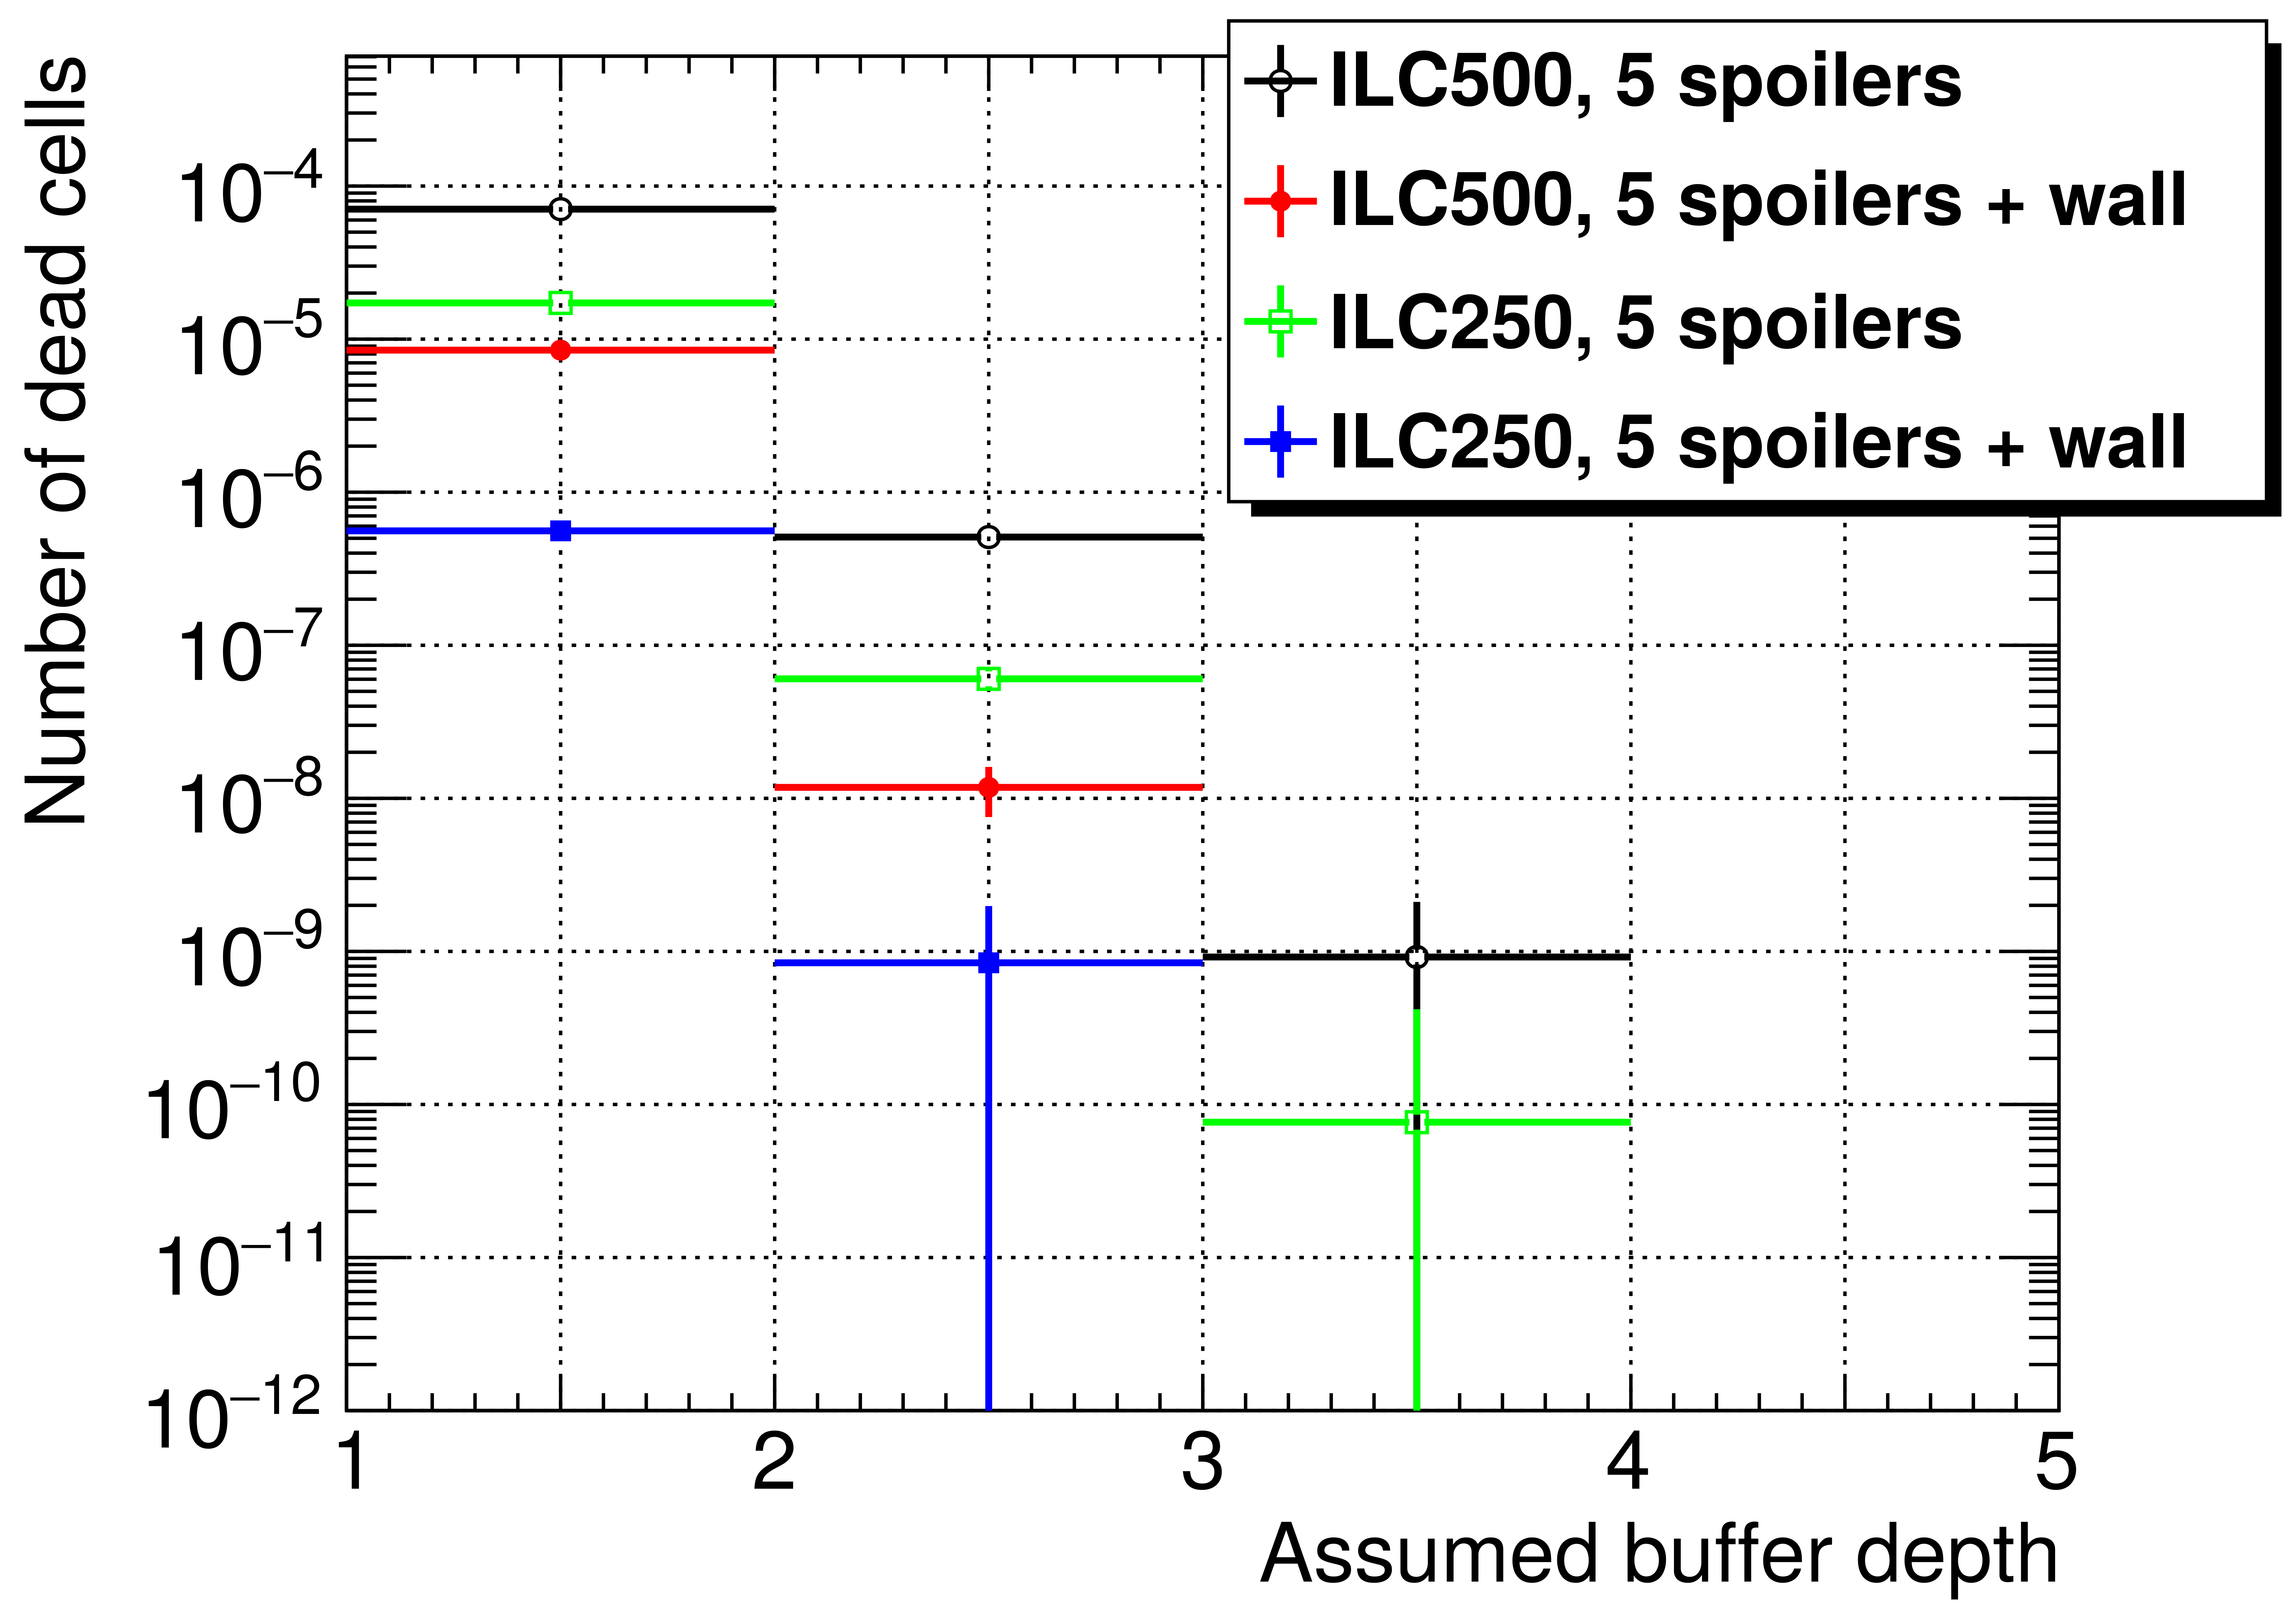
\includegraphics[width=\textwidth]{Figures/BDS_muons/Occupancy_Comparison_All_layers_deadcells_HcalBarrel.png}
   \caption{Normalized number of dead cells}
   \end{subfigure}
   \caption[\sid HCAL barrel occupancy from BDS muons]{Subfigure (a) shows the muon occupancy in the \sid HCAL barrel after a full bunch train, whilst subfigure (b) shows the fraction of dead cells resulting from this occupancy.
   Both histograms are normalized by the total number of cells in the HCAL barrel.
   The first bin of Subfigure (a) contains the total number of cells, because of which the value of this bin is 1 for all cases.
   \\The dashed pink lines in Subfigure (b) indicate the the buffer depth of four for the current sensor design, and the guideline of \num{e-4} for a critical acceptance limit.}
   \label{fig:BDS_Muons:HcalBarrel}
 \end{figure}
\\For the \sid tracker endcaps, however, the number of hits per cell reaches a maximum of 30 (see Figure~\ref{fig:BDS_Muons:SiTrackerEndcap}).
As for the \sid tracker, a readout cell size of \SI{50}{\micro\meter}$\times$\SI{50}{\micro\meter} was assumed, this is at first not to be expected.
The total number of hits in the tracker is smaller than in the HCAL, and yet the number of hits per cell reaches a much larger value.
The reason for this is that low energy (of the order of several hundred MeV) muons spiral in the magnetic field of the detector solenoid magnet, and by doing so hit the active layer of the tracker endcap several times.
An example of a loop performed by such a muon is depicted in Figure~\ref{fig:BDS_Muons:loop}.
Although the number of hits per cell ranges up to 30, the occupancy is consistently below \num{e-6} for all cases.
The number of dead cells, shown in Figure~\ref{fig:BDS_Muons:SiTrackerEndcap} (b), is plotted as a function of an assumed buffer depth of up to 30 accordingly.
Assuming the sensors in the \sid tracker will have a buffer depth of four, about \num{2e-8} of all cells would be dead for the ILC500 with the ``5 spoilers'' shielding only.
Also in this subdetector, the muon occupancy is below the critical limit for \sid for any buffer depth that might be chosen as the sensor design.
\\In the ILC500 stage, the occupancy for all subdetectors is reduced by at least a factor of five when adding a magnetized wall to the muon shielding.
This factor is even higher in the ILC250 stage.
Plots of the occupancy for the remaining \sid subdetectors can be found in Appendix~\ref{Appendix:BDS_Muons}.
  \begin{figure}
 \centering
  \begin{subfigure}[b]{0.49\textwidth}
   \centering
    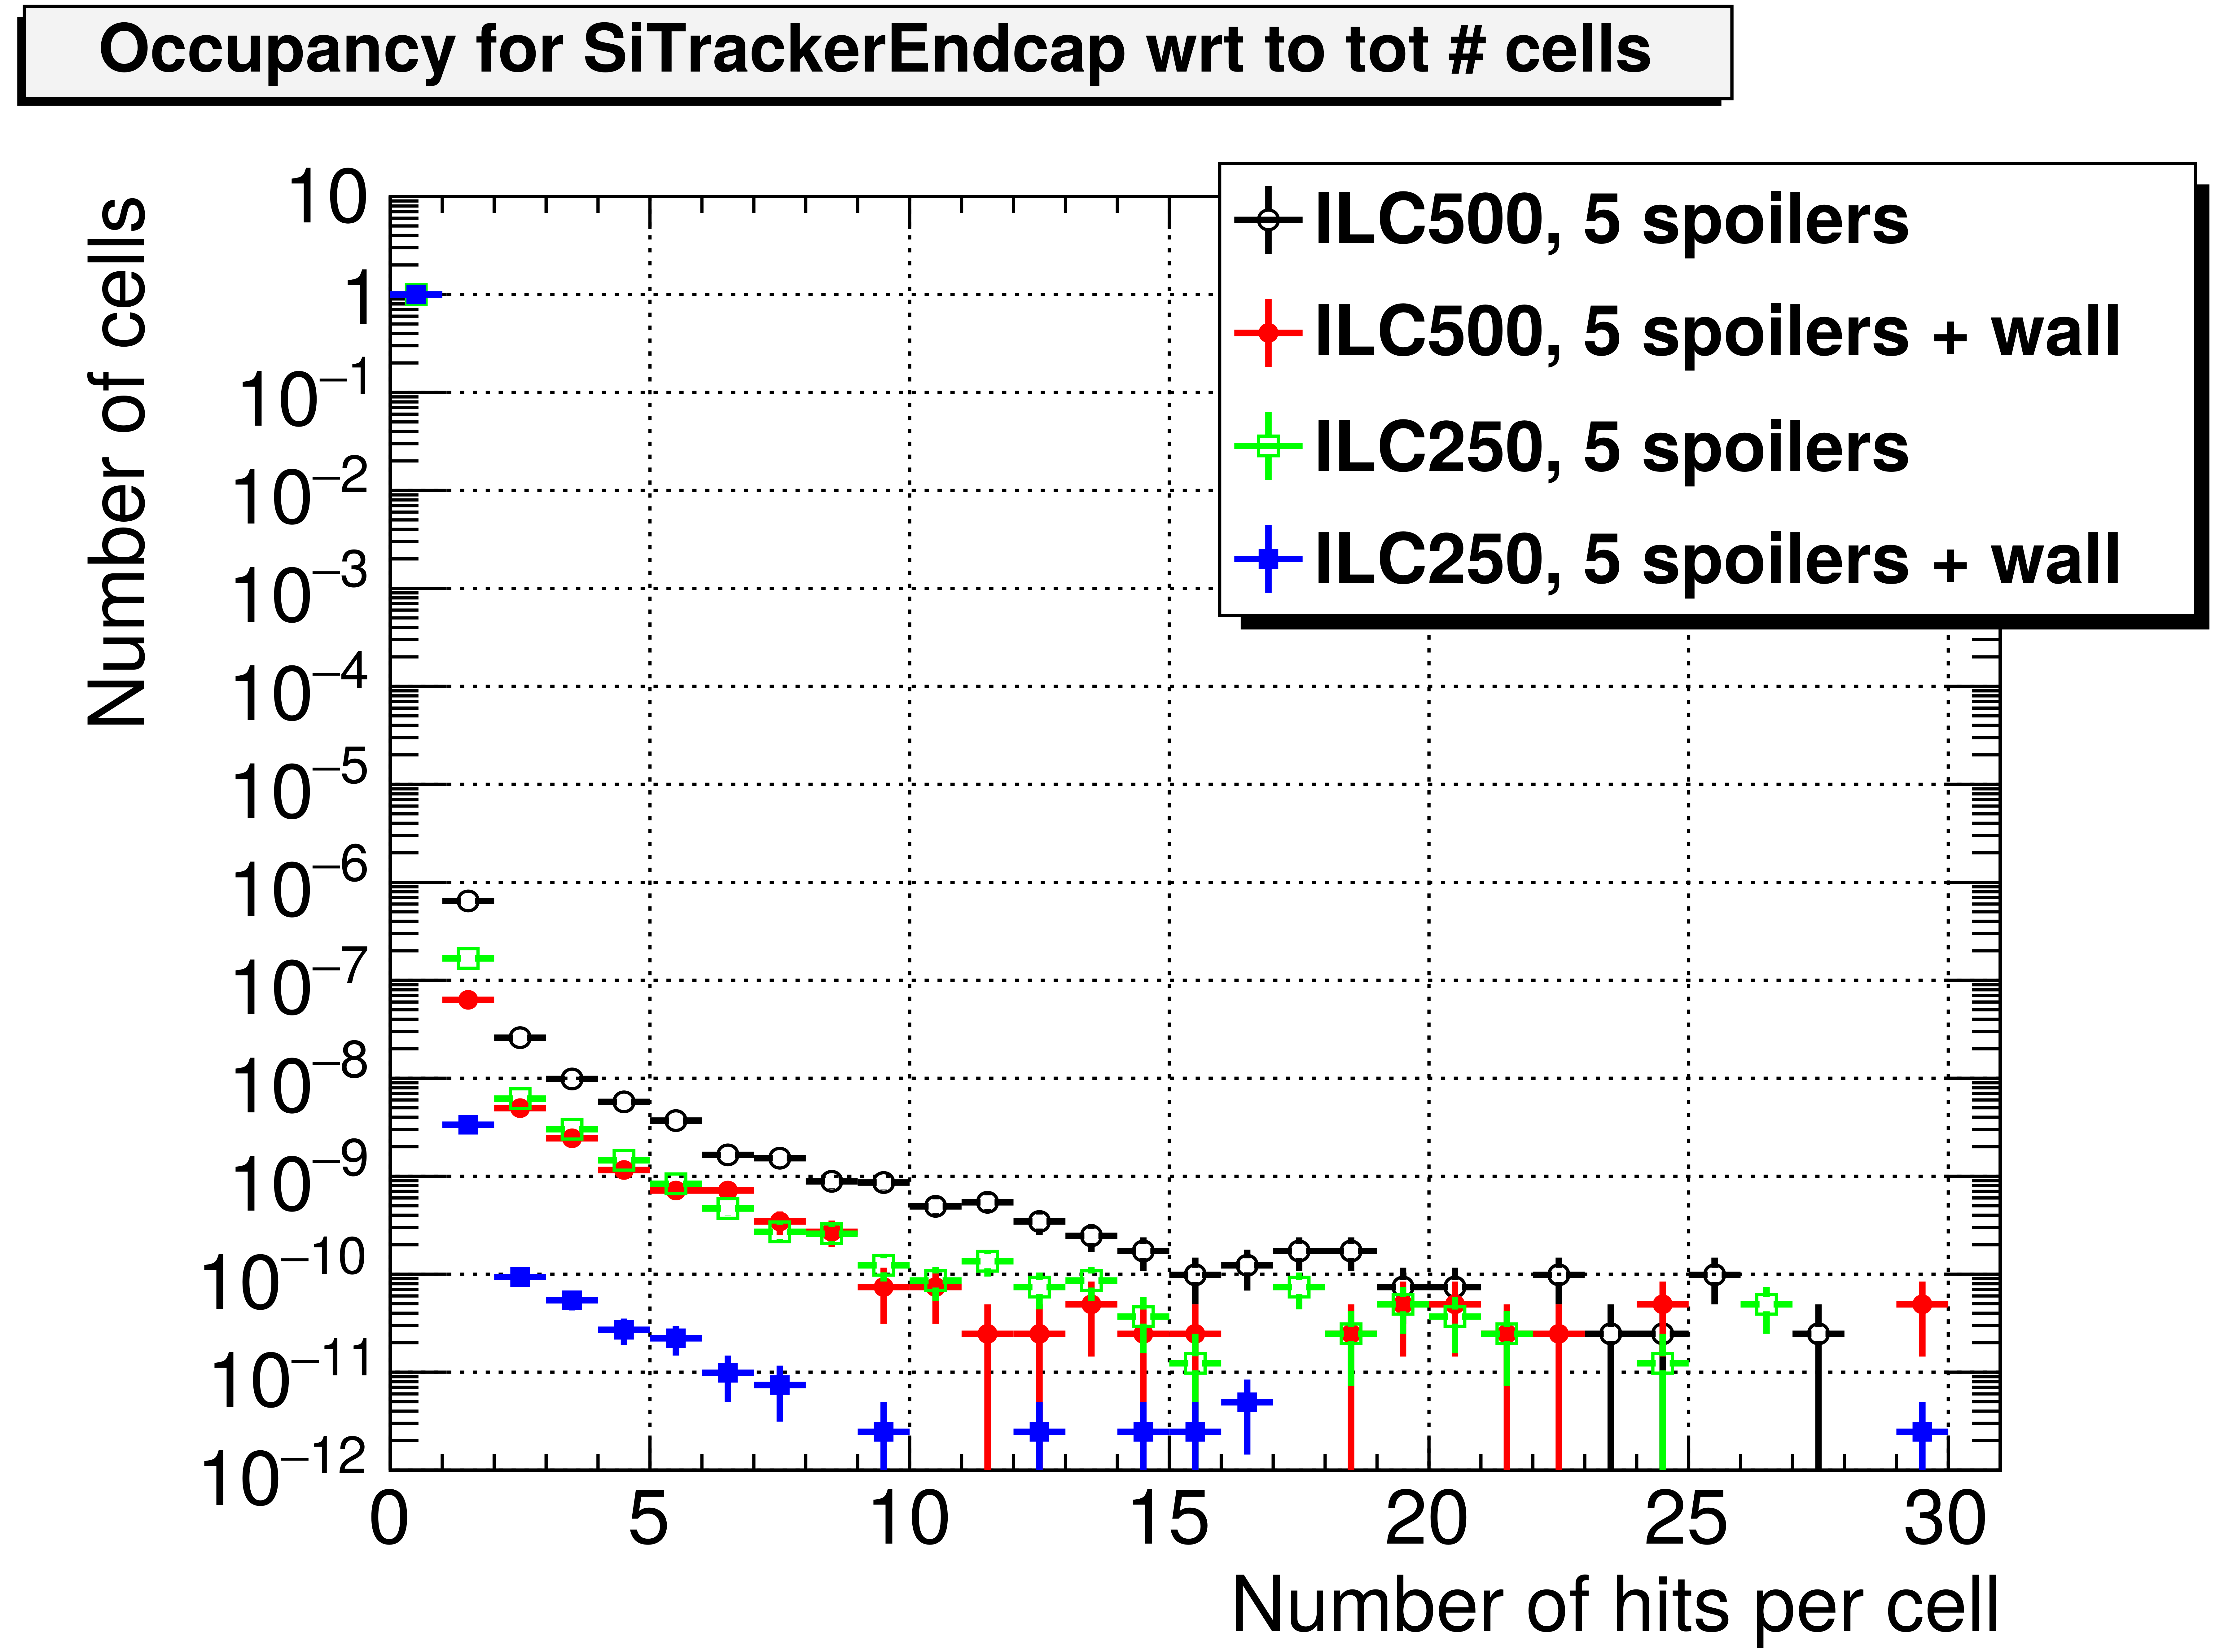
\includegraphics[width=\textwidth]{Figures/BDS_muons/Occupancy_Comparison_All_layers_wrt_cells_SiTrackerEndcap.png}
   \caption{Normalized occupancy}
   \end{subfigure}
   \hfill
    \begin{subfigure}[b]{0.49\textwidth}
   \centering
    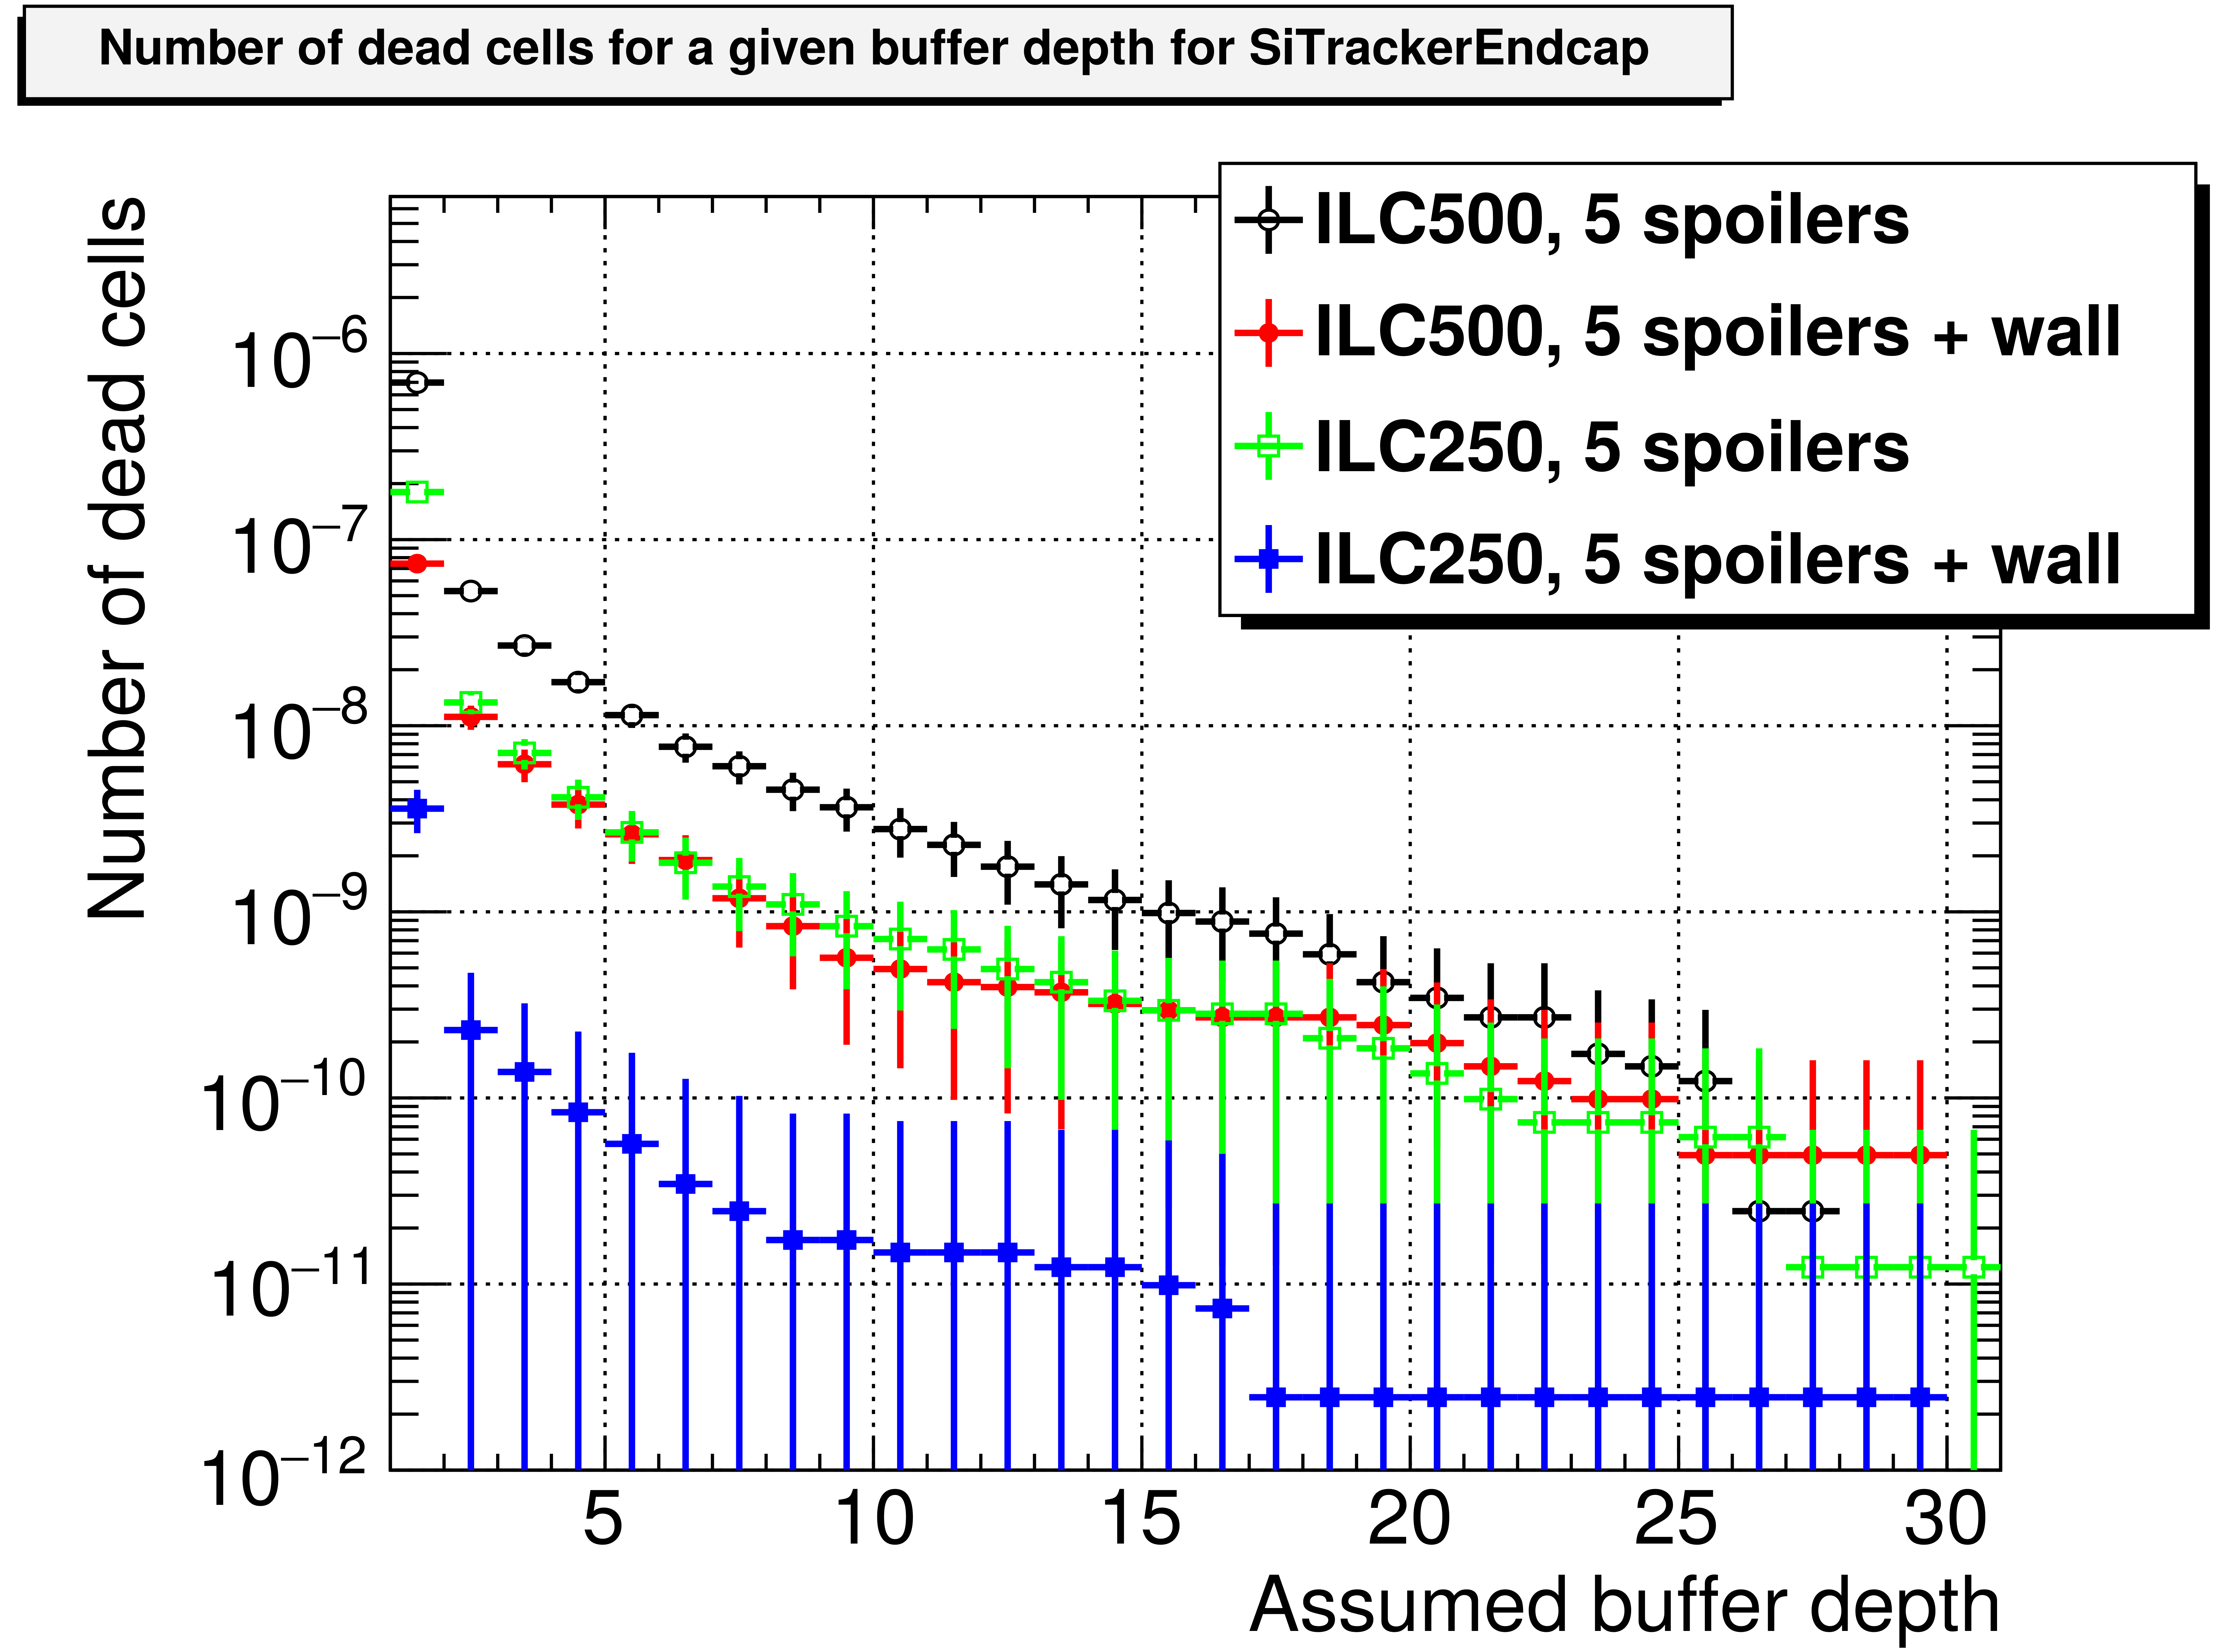
\includegraphics[width=\textwidth]{Figures/BDS_muons/Occupancy_Comparison_All_layers_deadcells_SiTrackerEndcap.png}
   \caption{Normalized number of dead cells}
   \end{subfigure}
   \caption[\sid tracker endcap occupancy from BDS muons]{Subfigure (a) shows the muon occupancy in one of the \sid tracker endcaps after a full bunch train, whilst subfigure (b) shows the fraction of dead cells resulting from this occupancy.
   Both histograms are normalized by the total number of cells in the tracker endcap.
   The first bin of Subfigure (a) contains the total number of cells, because of which the value of this bin is 1 for all cases.
   \\The dashed pink lines in Subfigure (b) indicate the the buffer depth of four for the current sensor design, and the guideline of \num{e-4} for a critical acceptance limit.}
   \label{fig:BDS_Muons:SiTrackerEndcap}
 \end{figure}
 
 \begin{figure}[htbp!]
\centering
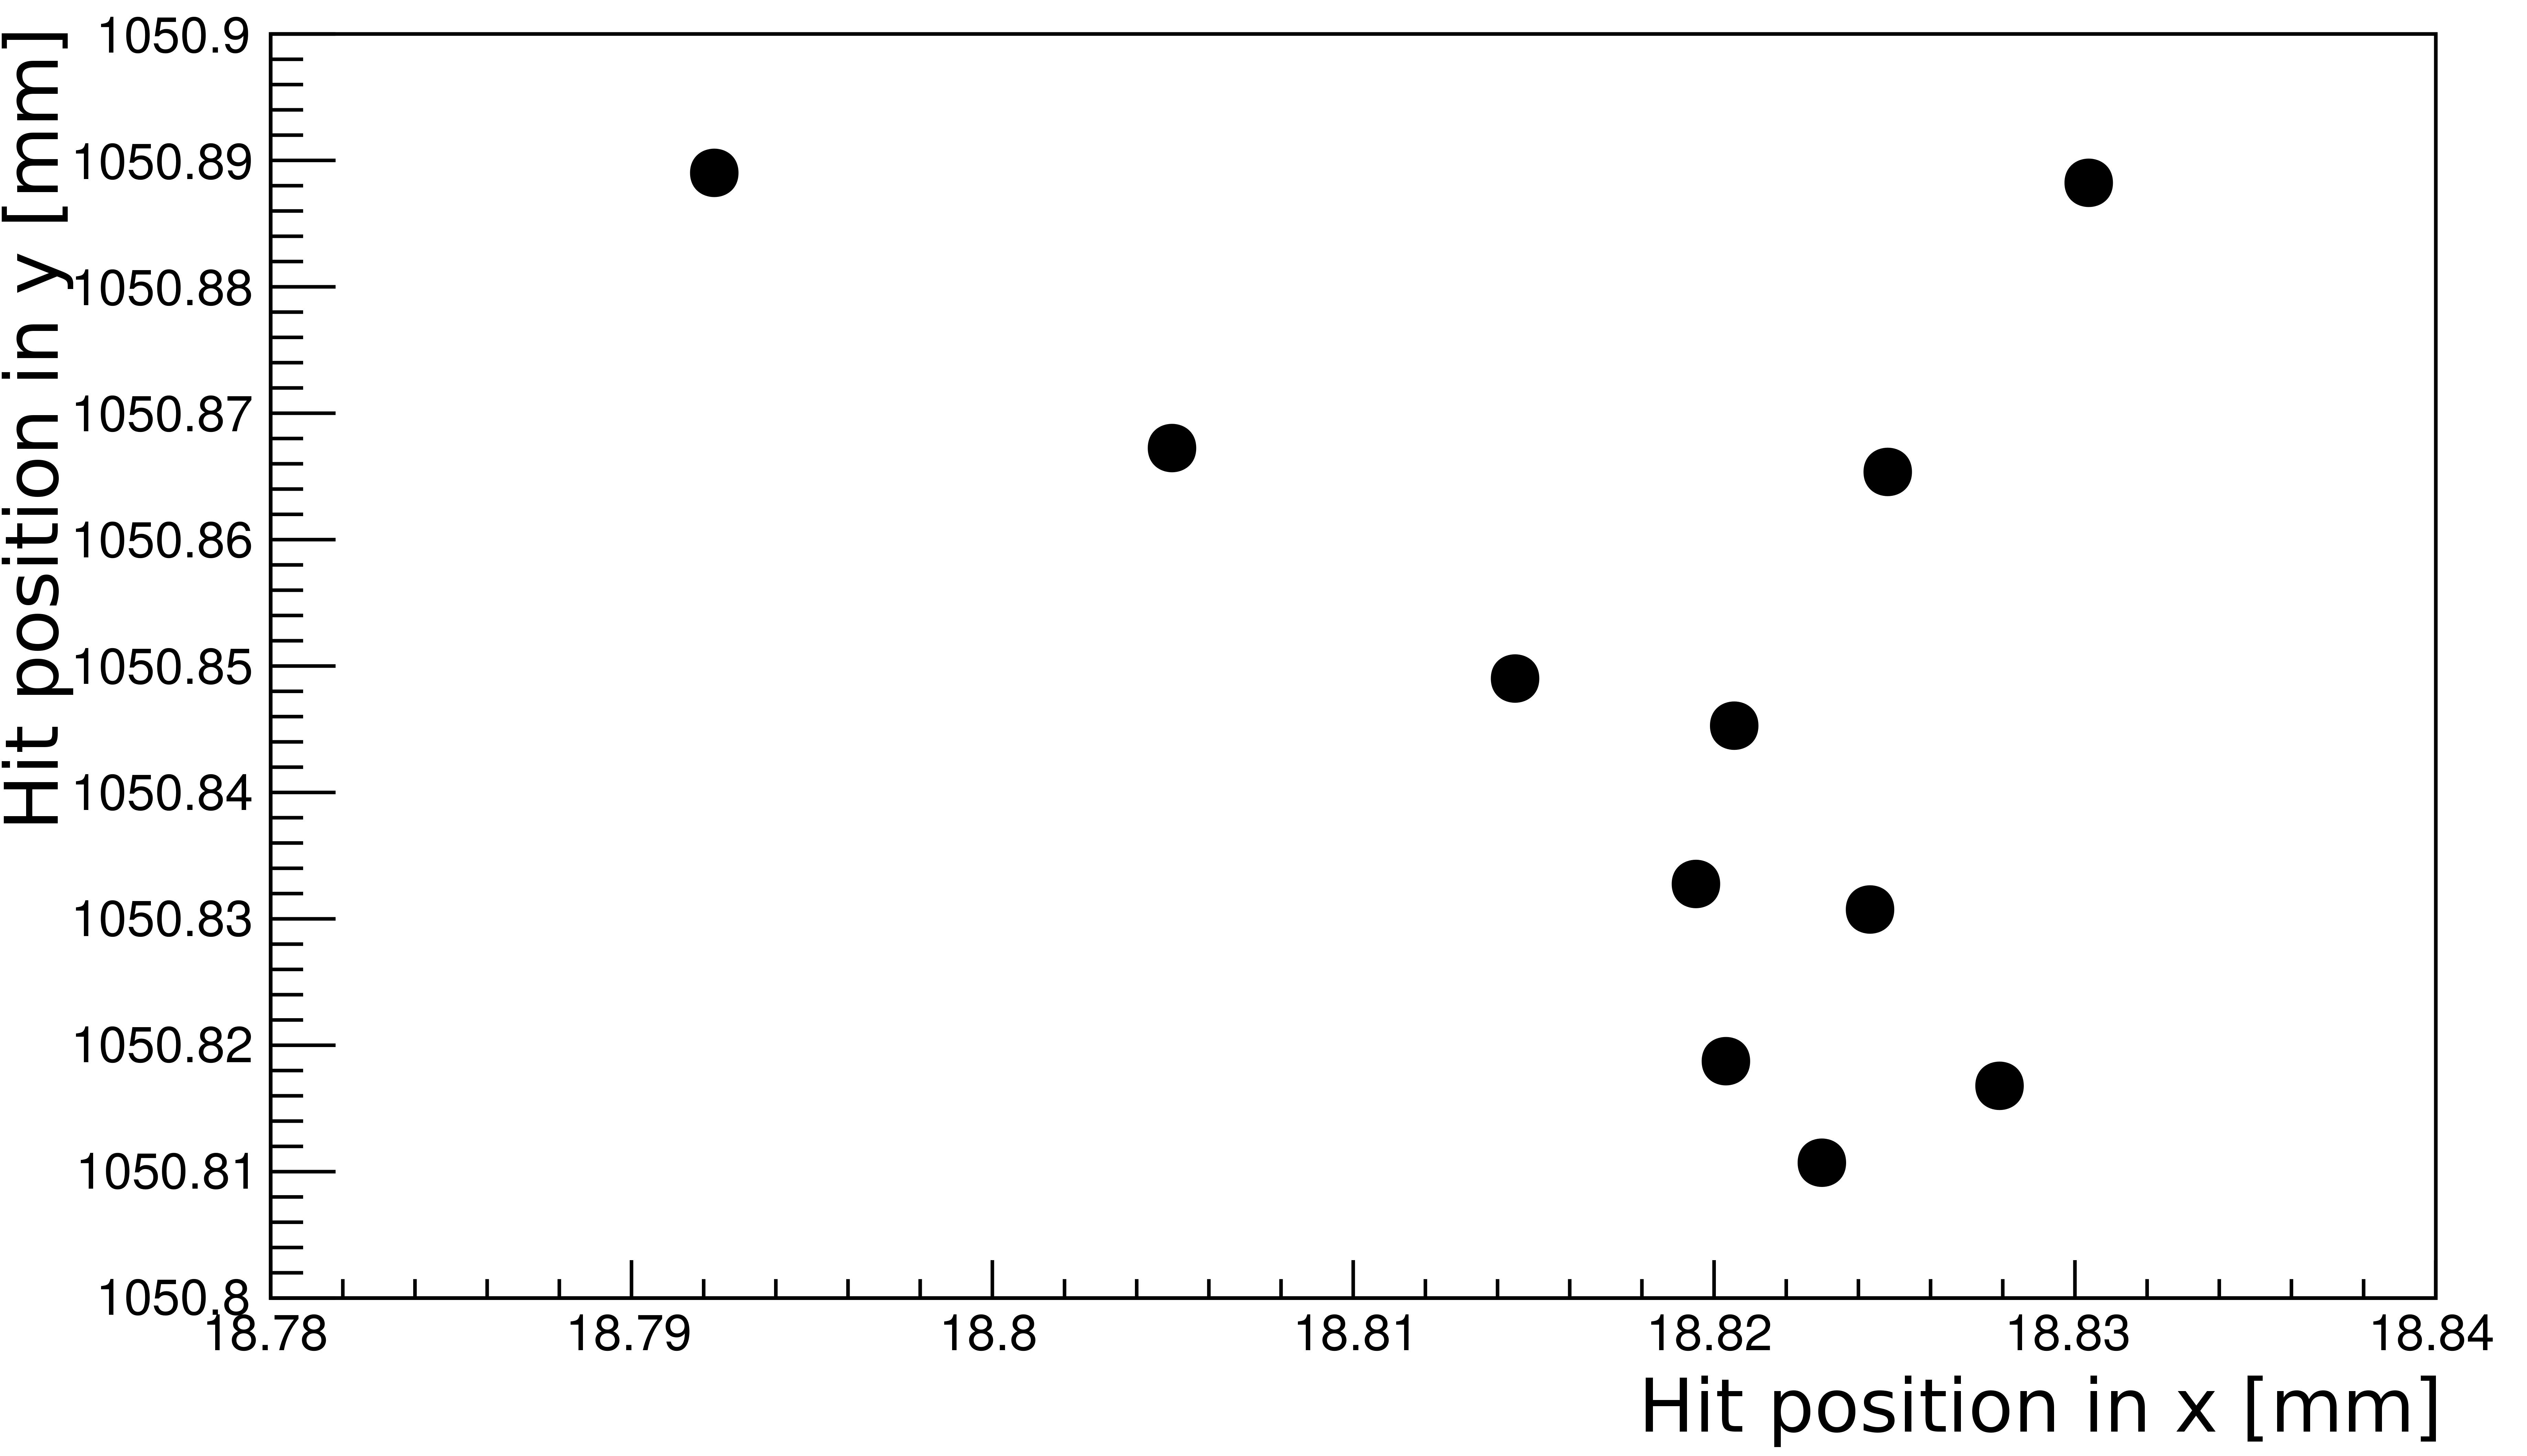
\includegraphics[width=0.5\textwidth]{Figures/BDS_muons/LoopInACell.png}
\caption[BDS muons looping]{Hit position of muon hits in the \sid tracker endcap, in layer number four.}
\label{fig:BDS_Muons:loop}
\end{figure}

\section{Conclusion}
This section presented a study of the effect of the muons from the BDS on the \sid occupancy for two different shielding options.
For the first option, five magnetized spoilers would be installed at different locations along the beam line.
For the second option, a magnetized wall would be placed between these spoiler locations and the interaction region, as an additional shielding device.

In Section~\ref{BDS_Muons:sidocc}, the comparison of the occupancy in these two cases revealed that the magnetized wall reduces the occupancy by a significant amount.
Nevertheless, the occupancy level is in both cases far from the critical limit of \num{e-4}, which is especially important in the tracking systems of the \sid detector.
For these subdetectors, a minimal background occupancy is crucial to guarantee a high performance in the track reconstruction of physics events.
For the first ILC stage, the \sid tracker endcap occupancy for an assumed buffer depth of four is about \num{4e-9} for the minimal shielding option without the wall.
Since in the next ILC stage at a center-of-mass energy of \SI{500}{\GeV}, the number of muons reaching the detector is larger by a factor of three, also the occupancy for the same buffer depth is increased by about a factor of three for the ``5 spoilers'' case.
However, it still does not exceed \num{e-7}.
\\The total number of muons produced in the BDS in both of the studied ILC stages is listed in Table~\ref{tab:BDS_Muons_muon_numbers}.

Overall, the magnetized wall does not seem to be necessary in order to limit the muon occupancy in \sid, for both studied center-of-mass energies.
However, the wall serves as a tertiary containment device against muons and other machine background particles.
The decision might be to keep the wall anyway for the protection of personnel and maintenance staff, depending on the restrictions imposed by radiation safety regulations.
A solution to lessen the price for the wall would be to change its design such that its thickness is reduced and it is not magnetized.
The wall would then still serve as additional shielding but does not deflect charged particles. \\The next step for the studies of the muon shielding would be to also adjust the detector specific Pacman design with respect to different materials and the possibility of magnetizing the Pacman volume.

Additionally, the timing of the muons (discussed in Section~\ref{BDS_Muons:hit_time_dis}) gives reason to study possible time gates in the individual subdetectors.
Since the muons hit the muon system first and then penetrate the inner subdetectors, there are distinct hit times.
Specific time gates for each subdetector could be decided on, in order to reduce the background occupancy.